% ============================================================
%  第五卷 第二章 热力学量（§9–§27 + 习题）
%  底本：高教社中文版第5版（束仁贵/束莼 译，郑伟谋 校）
%  OCR/原书错误已按 原书转换/pages/p-044…p-082.png 逐页核实修正：
%   1. (9.2) OCR "S=k ln ΔT"→原书 S=k ln ΔΓ（统计权重，p-045）；
%      (9.3) 箭头丢失，按原书补 T→kT、S→S/k。
%   2. (10.2) 右端 OCR 乱码（"λ_b/ℏ ∂ξ/∂λ χ"），原书两处均为"=常数"（p-045）；
%      (10.3) 竖线括号按原书为花括号求和式；§10 角速度两处 OCR \mathscr{a}→Ω。
%   3. §11 "热力学能量 E=E(p,q;λ)" 原书有平均线 E=\overline{E(p,q;λ)}（p-048）；
%      (11.3) 左端、(11.4) 左端 \overline{∂Ĥ/∂λ} 平均线 OCR 丢失，按 p-049 补回。
%   4. §14 "称为物体的焓②" 圈码② OCR 丢失，按 p-054 补回；
%      (14.7) OCR 未给编号，但 (18.2) 引用"(14.7)"式，按原书编号。
%   5. (15.10) 后 dF 式与正文 Λ_i，OCR 误作 A_i，统一为 \Lambda_i；
%      (15.12) OCR \mathfrak{E}→δ；§15 "（这时必须记住，…应看作为常数"原书缺
%      右括号，补"）"（p-056）。
%   6. §16 雅可比行列式链（C_v=C_p−T…）第三行首项 OCR "C_v"按原书为 C_p，
%      第二行各偏导下标按 p-059 还原；(16.13)–(16.16) 原书熵下标 S 大小写不一
%      （(16.12) 用小写 s，(16.13)–(16.16) 用大写 S），全章统一为小写斜体 s；
%      (16.7)(16.8) 原书两式并列一行，因版心宽度分排两行（编号不变）。
%   7. §18 "（图2的a）" OCR "图2的^{a)}"还原（p-062）。
%   8. §19 |δR|_max 链式 OCR 乱码，按 p-064 还原为
%      |δR|_max=−δE₁−δE₂=−T₁δS₁−T₂δS₂=−(T₂−T₁)δS₂。
%   9. §20 "竖直线段 ab" OCR 误作 bc，按 p-067 改正；总熵/总能下标统一为斜体 t。
%  10. §22 "而 y 为" OCR 误作 γ；"如果除了 ∂S/∂y=0 以外"的"了"OCR 乱码按原书
%      还原（p-070）；(22.7)(22.8)(22.9)(22.10)(22.11) 下标 y 与 Y=0 按 p-072。
%  11. §23 (23.1)–(23.4) 中文"当T=0时"按原书排入公式（OCR 乱码）；(23.4) 左端
%      为 (C_p−C_v)/C_p（p-074）。
%  12. (24.1) 尾部 OCR "^{*}" 为噪声，删（p-075 无此记号）。
%  13. §25 (25.1) "μ=常数"、流体静压 "P=常数−ρgz" 按 p-078 还原（OCR 乱码）。
%  14. §26 "根据同样的理由" OCR 窜入"μ₀"删（p-079）；E′、M 的平均线按 p-079 补回。
%  15. §27 (27.2)–(27.5) 中文"常数"按原书还原（OCR 乱码），(27.4) 结构为
%      "T=常数·dx⁰/ds，μ=常数·dx⁰/ds"（p-081）。
%  16. §9 "处于热力学平衡状态.那么"、§27 "（ε是…能量"两处原书排印缺/误标点，
%      分别改"，"与补"）"（p-044、p-082）。
%  17. 全章半角标点按文体约定改全角；V/ν/υ、C_ν/C_υ 等按下标约定统一：
%      C_v、C_p 小写；导数下标 v、s、p、w 小写，T、E、N 大写。
%  圈码脚注 25 处已全部还原为 \footnote（脚注代理转录，页面 p043–p082；
%  实际页码与脚注页码对照.txt 有三处 ±1 偏差：§12 脚注②实为 p050、
%  §27 脚注②实为 p081、§27 脚注③实为 p082。p044 ①与 p059 ①（雅可比
%  行列式定义及性质 (I)–(V)）脚注内含 equation* 展式，(I)–(V) 为脚注内
%  \tag 编号，与原书一致）。
%  遗留问题：
%   - (15.5)(17.1)(24.13)(24.14)(26.8) 等式尾标点版面不清，按 OCR 不加或照排。
% ============================================================
\chapter{热力学量}

\section{温度}

表征物体宏观状态的物理量称为热力学量.在热力学量中有一些量，不仅具有热力学的意义，而且也具有纯力学的意义.例如，能量与体积就是这样.但是还存在另外一类量，它们只是作为纯粹统计规律性的产物，而在应用于非宏观系统时就没有意义，例如熵.

以后我们要引入热力学量之间的一系列关系式，这些关系式总是成立的，与热力学量究竟属于什么样的实际物体无关.这些关系式称为热力学关系式.

在运用热力学量的时候，通常对它们经历的微小的涨落并不感兴趣.因此，我们将完全忽略这些涨落，仅仅在物体的宏观状态改变的情况下才考虑热力学量怎样变化\footnote{热力学量的涨落将在第十二章专门讨论.}.

考虑彼此处于热平衡的两个物体，并且这两个物体一起组成一个闭合系统.那么这个系统的熵$S$（在系统能量给定为$E$的情况下）有最大的可能值.能量$E$是每个物体的能量$E_1$与$E_2$之和：$E=E_1+E_2$.系统的熵也是如此，而且每个物体的熵都是各自能量的函数：$S=S_1(E_1)+S_2(E_2)$.因为$E_2=E-E_1$，其中$E$是常数，所以$S$实际上是单个自变量的函数，极大值的必要条件可以写成
\begin{equation*}
  \frac{\mathrm{d}S}{\mathrm{d}E_1}
  =\frac{\mathrm{d}S_1}{\mathrm{d}E_1}
  +\frac{\mathrm{d}S_2}{\mathrm{d}E_2}\frac{\mathrm{d}E_2}{\mathrm{d}E_1}
  =\frac{\mathrm{d}S_1}{\mathrm{d}E_1}
  -\frac{\mathrm{d}S_2}{\mathrm{d}E_2}=0,
\end{equation*}
由此，
\begin{equation*}
  \frac{\mathrm{d}S_1}{\mathrm{d}E_1}=\frac{\mathrm{d}S_2}{\mathrm{d}E_2}.
\end{equation*}
该结论不难推广到任意多个物体彼此处于平衡的情况.

由此可见，如果系统处于热力学平衡状态，那么熵对能量的导数，对于系统中所有各部分都是相同的，即在整个系统内都不变.物体的熵$S$对其能量$E$的导数的倒数称为该物体的绝对温度，或简称温度$T$
\begin{equation}
  \frac{\mathrm{d}S}{\mathrm{d}E}=\frac{1}{T}
\end{equation}
因此彼此处于平衡的物体的温度是相等的，$T_1=T_2$.

正如熵一样，温度显然也是一个纯粹统计性质的量，只对宏观物体才有意义.

其次，我们考虑彼此组成闭合系统，但并不处于平衡状态的两个物体.它们的温度$T_1$和$T_2$是不同的.随着时间的推移，在这两个物体之间将建立起平衡状态，并且它们的温度将逐渐趋于相等.同时它们的总熵$S=S_1+S_2$应该增加，即熵对时间的导数是正的：
\begin{equation*}
  \frac{\mathrm{d}S}{\mathrm{d}t}
  =\frac{\mathrm{d}S_1}{\mathrm{d}t}+\frac{\mathrm{d}S_2}{\mathrm{d}t}
  =\frac{\mathrm{d}S_1}{\mathrm{d}E_1}\frac{\mathrm{d}E_1}{\mathrm{d}t}
  +\frac{\mathrm{d}S_2}{\mathrm{d}E_2}\frac{\mathrm{d}E_2}{\mathrm{d}t}>0.
\end{equation*}
因为总能量保持守恒，所以
$\dfrac{\mathrm{d}E_1}{\mathrm{d}t}+\dfrac{\mathrm{d}E_2}{\mathrm{d}t}=0$，因此
\begin{equation*}
  \frac{\mathrm{d}S}{\mathrm{d}t}
  =\left(\frac{\mathrm{d}S_1}{\mathrm{d}E_1}
  -\frac{\mathrm{d}S_2}{\mathrm{d}E_2}\right)\frac{\mathrm{d}E_1}{\mathrm{d}t}
  =\left(\frac{1}{T_1}-\frac{1}{T_2}\right)\frac{\mathrm{d}E_1}{\mathrm{d}t}>0.
\end{equation*}
设第二个物体的温度高于第一个物体的温度（$T_2>T_1$）.考虑到温度是正的（参见下节），那么有
$\dfrac{\mathrm{d}E_1}{\mathrm{d}t}>0$（相应地
$\dfrac{\mathrm{d}E_2}{\mathrm{d}t}<0$）.换句话说，第二个物体的能量减小，而第一个物体的能量增加.温度的这一性质可以这样表述：能量从温度较高的物体转移到温度较低的物体.

熵$S$是个无量纲量.因此从定义(9.1)得出，温度具有能量的量纲，所以就可以用能量的单位来量度，例如用尔格（erg）.但是，在普通条件下尔格似乎是太大的量，实际上通常用一种特殊的单位来量度温度，这种单位称为开尔文（K），或简称为开.尔格与开尔文之间的变换系数，即每一开尔文的尔格数，称为玻尔兹曼常量，通常用字母$k$表示，它等于\footnote{为便于查询，我们也给出开尔文（K）与电子伏特（eV）之间的换算系数：
\begin{equation*}
  1\ \mathrm{eV}=11606\ \mathrm{K}.
\end{equation*}}
\begin{equation*}
  k=1.38\times10^{-16}\ \mathrm{erg/K}
\end{equation*}
我们约定今后所有的公式中温度都以能量为单位来量度.如果在数值计算时，要将温度换算成以开尔文来量度，只需用$kT$替换$T$.因子$k$只是用于标示温度的单位约定，处处记$k$只会让公式繁冗.

如果温度以开尔文为单位，为避免在普遍的热力学关系式中出现常数$k$，通常也在熵的定义中引入因子$k$，写成
\begin{equation}
  S=k\ln\Delta\Gamma
\end{equation}
以取代(7.7)式.那么定义温度的公式(9.1)，以及本章下面导出的含温度的一切普遍热力学关系式在换算为开尔文时都不改变.

这样，换算为开尔文的规则就在于在所有公式中作代换
\begin{equation}
  T\to kT,\qquad S\to\frac{S}{k}
\end{equation}

\section{宏观运动}

物体的各个宏观部分作为整体参与的运动称为宏观运动，以区别于分子的微观运动.现在我们考虑在热力学平衡状态下宏观运动的可能性问题.

把物体划分为大量很小的（但是宏观的）部分，并设$M_a$、$E_a$和$\boldsymbol{P}_a$分别表示第$a$个部分的质量、能量和动量.每一部分的熵$S_a$是其内能的函数，即是它的总能量$E_a$与它的宏观运动的动能$P_a^2/2M_a$之差的函数\footnote{物体的熵只是它的内能的函数，这个事实可直接从伽利略相对性原理得出；量子态的数目、从而统计权重（其对数等于熵）在所有的惯性参考系也包括物体在其中是静止的参考系中，应该是同样的.}.因此物体的总熵可写成
\begin{equation}
  S=\sum_a S_a\left(E_a-\frac{P_a^2}{2M_a}\right).
\end{equation}
我们假设物体是闭合的.那么除了物体的能量守恒而外，物体的总动量与总角动量也是守恒的：
\begin{equation}
  \sum_a\boldsymbol{P}_a=\text{常数，}\qquad
  \sum_a\boldsymbol{r}_a\times\boldsymbol{P}_a=\text{常数}
\end{equation}
（$\boldsymbol{r}_a$是物体的第$a$个部分的径矢）.在平衡状态中，物体的总熵$S$作为动量$\boldsymbol{P}_a$的函数，在附加条件(10.2)下具有极大值.根据熟知的拉格朗日不定乘子法，使和式
\begin{equation}
  \sum_a\left\{S_a+\boldsymbol{a}\cdot\boldsymbol{P}_a
  +\boldsymbol{b}\cdot(\boldsymbol{r}_a\times\boldsymbol{P}_a)\right\},
\end{equation}
（式中$\boldsymbol{a},\boldsymbol{b}$为常矢量）对$\boldsymbol{P}_a$的导数等于零，我们求出总熵为极大值的必要条件.把$S_a$对$\boldsymbol{P}_a$进行求导\footnote{标量对矢量的微商应理解为这样一个矢量：其分量等于标量对于该矢量的诸分量的微商.}，再根据温度的定义，就给出
\begin{equation*}
  \frac{\partial}{\partial\boldsymbol{P}_a}
  S_a\left(E_a-\frac{P_a^2}{2M_a}\right)
  =-\frac{\boldsymbol{P}_a}{M_aT}=-\frac{\boldsymbol{v}_a}{T}
\end{equation*}
（$\boldsymbol{v}_a=\boldsymbol{P}_a/M_a$是物体的第$a$个部分的速度）.因此，(10.3)对$\boldsymbol{P}_a$求导，得
\begin{equation*}
  -\frac{\boldsymbol{v}_a}{T}
  +\boldsymbol{a}+\boldsymbol{b}\times\boldsymbol{r}_a=0
\end{equation*}
或
\begin{equation}
  \boldsymbol{v}_a=\boldsymbol{u}
  +\boldsymbol{\Omega}\times\boldsymbol{r}_a
\end{equation}
式中$\boldsymbol{u}=T\boldsymbol{a}$，$\boldsymbol{\Omega}=T\boldsymbol{b}$都是常矢量.

所得到的结果具有简单的物理意义.如果物体所有各部分的速度都由(10.4)式确定，而式中$\boldsymbol{u}$和$\boldsymbol{\Omega}$对于所有各部分都是相同的，这就意味着：我们讨论的情形就是物体以不变的速度$\boldsymbol{u}$作整体的平动和以不变的角速度$\boldsymbol{\Omega}$作整体的转动.因此，我们得到一个重要的结论：在热力学平衡状态下，闭合系统只可能整体作匀速的平动和转动，任何一种内部的宏观运动在平衡状态中都是不可能的\footnote{为避免误解，我们提出这个规则的一个重要例外：超流的液氦不可能作为整体旋转.这个现象将在本教程的第九卷中考虑；在这里仅指出：所作的证明，并不适用于该情形，因为速度的分布依从附加条件（超流运动的有势性），应在该条件下寻求熵的极大值.}.

以后我们通常研究静止的物体，相应地，能量$E$就是物体的内能.

到目前为止，只利用了熵作为动量的函数取极大值的必要条件，还没有利用附加到熵的二阶导数上的充分条件.容易看出，后者引导出一个非常重要的结论：温度只可能是正的，$T>0$\footnote{温度 $T=0$（绝对零度）对应摄氏温标 $-273.15$℃.}.为此甚至不必实际算出二阶导数，只要进行如下讨论就够了.

考虑一个整体静止的闭合系统.假如温度会是负的，那么熵就会随着它的宗量的减小而增长.由于熵有增长的趋势，物体就会有自发地瓦解为相互飞散（同时保持总动量$\sum_a\boldsymbol{P}_a=0$）的各部分的趋势，以使和式(10.1)中的每一个$S_a$的宗量取尽可能小的数值.换句话说，在$T<0$时，根本不可能有平衡状态的物体存在.

不过在这里还应指出下述情况.虽然物体的温度或者它的任何一部分的温度从来不可能是负的，但是在不完全平衡状态下，负温度却被证明是可能的，在这种情况下与物体的一部分自由度相对应的温度可以是负的（详见§73）.

\section{绝热过程}

在物体所经受的各类外界作用中，有一种特殊类型的作用，其作用归结为改变物体所处的外界条件.我们把外界条件广义地理解为各种不同的外场.实际上，最常遇到的外界条件就是规定物体外形的体积.在某种意义下，这种情形也可以看成是一种特殊类型的外场，因为限制着体积的器壁，就其作用而言，等效于阻止物体的分子向外逃逸的势垒.

如果除了外界条件的改变以外，物体不再受到其它任何作用，就说物体是热绝缘的.应当强调：虽然热绝缘的物体与任何别的物体并无直接相互作用，但是一般来说，它并不是闭合的，而且它的能量可以随时间而变化.

从纯力学观点来看，热绝缘的物体不同于闭合物体之处就在于：由于存在着变化的外场，它的哈密顿函数（能量）明显地与时间有关：$E=E(\boldsymbol{p},\boldsymbol{q},t)$.假如物体与其它物体还直接发生相互作用，则它本身就完全不会有哈密顿函数，因为相互作用不仅仅与该物体分子的坐标有关，而且还与其它物体分子的坐标有关.

这种情况可以得出这样的结论：熵增长定律不仅对闭合系统是正确的，而且对热绝缘的物体也是正确的.实际上，在这里我们把外场看成是完全给定了的坐标和时间的函数，特别是忽略了物体自身对外场的反作用.换句话说，在这里场是纯力学的对象，而不是统计学的对象，因而在这种意义下也可以说：它的熵等于零.由此也就得出了上面作出的结论.

假设物体是热绝缘的，而且它所处的外界条件变化得足够缓慢，这样的过程称为绝热过程.我们要证明，在绝热过程中，物体的熵保持不变，即该过程是可逆的.

我们可以用一些参量来表征外界条件，这些参量都是时间的给定函数.例如，假设总共只有一个这样的参量，用字母$\lambda$来表示.熵对时间的导数$\dfrac{\mathrm{d}S}{\mathrm{d}t}$将以某种方式依赖于$\lambda$对时间的变化率$\dfrac{\mathrm{d}\lambda}{\mathrm{d}t}$.由于$\dfrac{\mathrm{d}\lambda}{\mathrm{d}t}$很小，可以把$\dfrac{\mathrm{d}S}{\mathrm{d}t}$展开成$\dfrac{\mathrm{d}\lambda}{\mathrm{d}t}$的幂级数.该展开式的零次项，即不含$\dfrac{\mathrm{d}\lambda}{\mathrm{d}t}$的项为零，因为处于热力学平衡状态的闭合系统，在不变的外界条件下其熵应该保持不变，所以当$\dfrac{\mathrm{d}\lambda}{\mathrm{d}t}=0$时，$\dfrac{\mathrm{d}S}{\mathrm{d}t}$也应该为零.可是与$\dfrac{\mathrm{d}\lambda}{\mathrm{d}t}$成正比的一阶项也应该为零.事实上，该项应该随着$\dfrac{\mathrm{d}\lambda}{\mathrm{d}t}$改变符号而变号.然而，根据熵增长定律，$\dfrac{\mathrm{d}S}{\mathrm{d}t}$总是正的.由此得出结论，$\dfrac{\mathrm{d}S}{\mathrm{d}t}$的展开式从二阶项开始，即当$\dfrac{\mathrm{d}\lambda}{\mathrm{d}t}$很小时有
\begin{equation*}
  \frac{\mathrm{d}S}{\mathrm{d}t}
  =A\left(\frac{\mathrm{d}\lambda}{\mathrm{d}t}\right)^2,
\end{equation*}
由此得到
\begin{equation*}
  \frac{\mathrm{d}S}{\mathrm{d}\lambda}
  =A\frac{\mathrm{d}\lambda}{\mathrm{d}t}.
\end{equation*}
因此，当$\dfrac{\mathrm{d}\lambda}{\mathrm{d}t}$趋近于零时，$\dfrac{\mathrm{d}S}{\mathrm{d}\lambda}$也趋近于零，这就证明了绝热过程的可逆性.

必须强调指出，虽然绝热过程是可逆的，但是绝非任何可逆过程都是绝热的.过程的可逆性条件只要求整个闭合系统的总熵不变，而它的各个部分的熵既可以增加，也可以减少.但是在绝热过程的情况下，必须满足一个更为严格的条件：对于给定的物体虽然本身只是闭合系统的一个组成部分，但是其熵也必须保持不变.

以上我们把绝热过程定义为足够缓慢的过程.更确切地说，外界条件必须变化得如此缓慢，以致在每一时刻都可以认为，物体是处在与该时刻所存在的外界条件相对应的平衡状态之中.换句话说，绝热过程必须比在该物体中建立平衡状态的过程更加缓慢.\footnote{事实上，该条件可能是很不严格的，也就是说“缓慢”的绝热过程实际上可能进行得相当“迅速”.例如，在气体膨胀时（比如活塞在汽缸中向外移动）活塞的速度只要比气体中的声速小得多就可以，即在实际上它可能还是很大的.
在物理学的一般教程中，绝热膨胀（或压缩）常常被定义为“非常迅速的”.这时候，所注意的是问题另一方面——过程应该进行得如此迅速，以使物体来不及与周围介质进行热交换.由此可见，我们所注意的是能够实际保证物体的热绝缘性条件，而应当比建立平衡状态的过程缓慢得多这一条件就默认为已经满足了.}

我们来推导一个公式，该公式使得通过纯热力学的途径能够计算各种平均值.为此，假定物体经历着一个绝热过程，我们要确定物体的能量对时间的导数$\dfrac{\mathrm{d}E}{\mathrm{d}t}$.根据定义，热力学能量$E=\overline{E(p,q;\lambda)}$，其中$E(p,q;\lambda)$是物体的哈密顿函数，它以$\lambda$作为参变量.从力学已经知道（参看第一卷§40），哈密顿函数对时间的全导数就等于它对时间的偏导数
\begin{equation*}
  \frac{\mathrm{d}E(p,q;\lambda)}{\mathrm{d}t}
  =\frac{\partial E(p,q;\lambda)}{\partial t}.
\end{equation*}
在给定的情况下，$E(p,q;\lambda)$通过$\lambda(t)$而明显地与时间有关，所以能够写成
\begin{equation*}
  \frac{\mathrm{d}E(p,q;\lambda)}{\mathrm{d}t}
  =\frac{\partial E(p,q;\lambda)}{\partial\lambda}
  \frac{\mathrm{d}\lambda}{\mathrm{d}t}.
\end{equation*}
因为按照统计分布求平均值的运算与对时间求导的运算显然可以按任意次序进行，我们有
\begin{equation}
  \frac{\mathrm{d}E}{\mathrm{d}t}
  =\overline{\frac{\mathrm{d}E(p,q;\lambda)}{\mathrm{d}t}}
  =\overline{\frac{\partial E(p,q;\lambda)}{\partial\lambda}}
  \frac{\mathrm{d}\lambda}{\mathrm{d}t}
\end{equation}
（导数$\mathrm{d}\lambda/\mathrm{d}t$是给定的时间函数，因而可以从平均号下提出来）.

更重要的，由于绝热过程，式(11.1)中的导数$\dfrac{\partial E(p,q;\lambda)}{\partial\lambda}$的平均值可以理解为按统计分布求平均，该统计分布与在参量$\lambda$的给定值下的平衡状态相对应，即与该时刻所存在的外界条件下的平衡状态相对应.

把热力学量$E$看成物体的熵$S$和外参量$\lambda$的函数，就可以把导数$\dfrac{\mathrm{d}E}{\mathrm{d}t}$写成另外的形式.因为在绝热过程中熵$S$保持不变，所以我们有
\begin{equation}
  \frac{\mathrm{d}E}{\mathrm{d}t}
  =\left(\frac{\partial E}{\partial\lambda}\right)_s
  \frac{\mathrm{d}\lambda}{\mathrm{d}t},
\end{equation}
式中括号下方的字母表明导数是在$S$不变的情况下取的.

将式(11.1)与式(11.2)相比较，我们得到：
\begin{equation}
  \overline{\frac{\partial E(p,q;\lambda)}{\partial\lambda}}
  =\left(\frac{\partial E}{\partial\lambda}\right)_s,
\end{equation}
这就是所求的公式.该公式使得能够通过热力学的途径来计算形为
$\overline{\dfrac{\partial E(p,q;\lambda)}{\partial\lambda}}$的量（按照平衡的统计分布）的平均值.这种类型的量在研究宏观物体的性质时常会遇到，因此(11.3)式在统计学中起着非常重要的作用.计算作用于物体上的各种力（这时作为参量$\lambda$的是物体某一部分的坐标，参阅下面讨论压强的一节），计算物体的磁矩或电矩（这时作为参量$\lambda$的是磁场强度或电场强度）等等，都属于这一类.

我们在这里对于经典力学的情形所进行的全部讨论也完全可以应用到量子理论中去，只需要在所有的地方都用哈密顿算符$\hat{H}$去代替能量$E(p,q;\lambda)$就行了.这时公式(11.3)写成如下形式
\begin{equation}
  \overline{\frac{\partial\hat{H}}{\partial\lambda}}
  =\left(\frac{\partial E}{\partial\lambda}\right)_s,
\end{equation}
式中横线表示完全的统计平均，该平均已自动包含了量子力学的平均.

\section{压强}

物体的能量$E$是一个可加性的热力学量：物体的能量等于它的各个（宏观的）部分的能量之和\footnote{其所以如此是由于我们忽略了这些部分之间的相互作用能；如果我们正是要考虑由于不同物体间存在着分界面而引起的那些现象（这些现象在第十五章中研究），就不能这样做了.}.另一个基本的热力学量熵也具有同样的性质.

能量和熵的可加性导致下列非常重要的结果.如果物体处于热平衡状态，那么可以断言：物体的熵在给定的能量值下（或物体的能量在给定的熵值下）仅与物体的体积有关而与物体的形状无关\footnote{这些论断事实上只适用于液体和气体，而不适用于固体，改变固体的形状（使之形变）要求耗费一定的功，即这时物体的能量被改变.这种情况是因为：固体的形变状态，严格地说，是不完全的热动平衡状态（但是为了建立完全平衡所需要的弛豫时间如此之大，以至于在很多方面，形变固体的行为都像在平衡状态一样）.}.实际上，物体形状的改变可以当成是物体各个部分的重新排列，由于熵与能量都是可加性量，所以它们不发生变化.当然，这时假定物体并不处于外力场中，所以物体各部分在空间的位移不至于引起它们能量的变化.

这样，处于平衡中的静止物体的宏观状态总共只要用两个量就可以完全确定，例如用体积与能量.所有其它的热力学量都可以表示为这两个量的函数.当然，因为各个热力学量之间的这种相互依赖关系，所以其它任何一对热力学量也都可以用来作为自变量.

现在我们来求物体作用于自身体积的边界上的力.根据力学中熟知的公式，作用到某个表面元$\mathrm{d}S$上的力等于
\begin{equation*}
  \boldsymbol{F}
  =-\frac{\partial E(\boldsymbol{p},\boldsymbol{q};\boldsymbol{r})}
  {\partial\boldsymbol{r}}
\end{equation*}
式中$E(\boldsymbol{p},\boldsymbol{q};\boldsymbol{r})$是物体的能量，作为物体中粒子的坐标与动量的函数，同时也作为该表面元的径矢的函数，在现在的情况下，面元的径矢起着外参量的作用.对该等式取平均值并利用(11.3)式，得到
\begin{equation*}
  \overline{\boldsymbol{F}}
  =-\overline{\frac{\partial E(\boldsymbol{p},\boldsymbol{q};\boldsymbol{r})}
  {\partial\boldsymbol{r}}}
  =-\left(\frac{\partial E}{\partial\boldsymbol{r}}\right)_s
  =-\left(\frac{\partial E}{\partial V}\right)_s
  \frac{\partial V}{\partial\boldsymbol{r}},
\end{equation*}
式中$V$为体积.因为体积的变化等于
$\mathrm{d}\boldsymbol{s}\cdot\mathrm{d}\boldsymbol{r}$，其中
$\mathrm{d}\boldsymbol{s}$是表面元，所以
$\dfrac{\partial V}{\partial\boldsymbol{r}}=\mathrm{d}\boldsymbol{s}$，因而
\begin{equation*}
  \overline{\boldsymbol{F}}
  =-\left(\frac{\partial E}{\partial V}\right)_s\mathrm{d}\boldsymbol{s}.
\end{equation*}
由此可见，作用在表面元上的平均力，指向该面元的法线方向并与该面元的面积成正比（帕斯卡定律）.作用到单位表面积上的力，其绝对值等于
\begin{equation}
  P=-\left(\frac{\partial E}{\partial V}\right)_s
\end{equation}
该物理量称为压强.

在用(9.1)式来定义温度时，实质上是对不直接与任何其它物体相接触的物体而言的，特别是对不被任何外界介质所包围的物体而言的.在这种条件下，不必确定过程的特征，就可以讨论物体的能量和熵的变化.而在物体处于外界介质中（或被容器壁所包围）的普遍情况下，公式(9.1)必须规定得更明确些.

实际上，如果在变化的进程中，给定物体的体积发生变化，这就不可避免地会影响到同它相互接触的诸物体的状态，因而为了定义温度，我们必须同时考虑所有这些同它相互接触的物体（例如，把物体与放置它的容器一起考虑）.而如果我们想仅仅根据一个给定物体的热力学量来定义温度，就必须认为这个物体的体积没有改变.换句话说，温度定义为：在恒定体积下取物体的能量对其熵的导数
\begin{equation}
  T=\left(\frac{\partial E}{\partial S}\right)_v.
\end{equation}
等式(12.1)，(12.2)可以合在一起写成以下微分关系式
\begin{equation}
  \mathrm{d}E=T\,\mathrm{d}S-P\,\mathrm{d}V.
\end{equation}
这是最重要的热力学关系式之一.

彼此处于平衡的物体，其压强彼此相等.这甚至从以下事实就可直接得出：任何情况下的热平衡都以存在力学平衡为前提，换而言之，这些物体中任何两个物体的相互作用力（遍及它们的接触表面）应该相互抵消，即其绝对值相等而方向相反.

平衡时压强相等也可以从熵是极大值的条件推导出来，完全类似于我们在§9中证明温度相等那样.为此，考虑处于平衡状态的闭合系统的两个相互接触的部分.熵为极大值的必要条件之一是：熵相对于这两部分的体积$V_1$和$V_2$的变化，如果其它部分的状态保持不变（这也特指$V_1+V_2$之和保持不变），应取极大值.如果$S_1$和$S_2$表示这两部分的熵，则有
\begin{equation*}
  \frac{\partial S}{\partial V_1}
  =\frac{\partial S_1}{\partial V_1}
  +\frac{\partial S_2}{\partial V_2}\frac{\partial V_2}{\partial V_1}
  =\frac{\partial S_1}{\partial V_1}
  -\frac{\partial S_2}{\partial V_2}=0.
\end{equation*}
但是，由改写的关系式(12.3)
\begin{equation*}
  \mathrm{d}S=\frac{1}{T}\,\mathrm{d}E+\frac{P}{T}\,\mathrm{d}V
\end{equation*}
可以看出$\dfrac{\partial S}{\partial V}=\dfrac{P}{T}$，因此
$\dfrac{P_1}{T_1}=\dfrac{P_2}{T_2}$.由于平衡时温度$T_1$和$T_2$相同，所以我们由此得出所求的压强相等关系式：$P_1=P_2$.

必须注意，在建立热平衡的过程中，压强达到相等（即力学平衡）远比温度达到相等要快得多.因此，常常会遇到这样的情况，在整个物体的压强是常数时，而温度还不是常数.问题就在于：压强不恒定与存在未抵消的力有关，这些力导致出现宏观运动，宏观运动促使压强趋于相等的过程远比促使温度趋于相等的过程进行得快得多，因为温度趋于相等的过程与宏观运动无关.

容易看出，在任何平衡状态下，物体的压强应该是正的.实际上，当$P>0$时有
$\left(\dfrac{\partial S}{\partial V}\right)_E>0$，因而物体的熵只可能在物体膨胀时增加，然而这种膨胀又会受到它周围物体的阻碍.反之，当$P<0$时就会有
$\left(\dfrac{\partial S}{\partial V}\right)_E<0$，因而物体就必须自发地收缩，致使熵增长.

但是，温度为正的要求与压强为正的要求之间有本质的区别.具有负温度的物体是完全不稳定的，因而不可能存在于自然界中.而具有负压强的（不平衡的）状态在自然界中是可以实现的，虽然只具有有限度的稳定性.问题就在于：物体自发地收缩使它“脱离开”容器壁，或者在物体的内部形成空腔，即物体形成了新的表面；这种情况就导致在所谓亚稳态中实现负压强的可能性\footnote{关于亚稳态的定义，参看§21；关于负压强，也可参看(83.1)后的脚注.}.

\section{功和热量}

作用在物体上的外力可以对物体做功，根据普遍的力学规则，功定义为这些力与它们所引起的位移的乘积.这个功可以使物体进入宏观运动的状态（通常用于改变物体的动能），或使物体在外场中产生位移（例如在重力场中使物体升高）.然而最使我们感兴趣的情况是对物体做功的结果改变了物体的体积（即外力是对物体进行压缩，物体作为一个整体仍然保持静止）.

以后我们约定外力对已知物体做功$R$总认为是正的，负功$R<0$相应地表示已知物体本身（例如物体膨胀时）对某些外界客体做功（大小为$|R|$）.

作用在物体表面单位面积上的力是压强，而表面的面元与它的位移的乘积就是该面元运动所扫过的体积，注意到这两点我们就求得物体体积改变时对物体所做的功（在单位时间内）是
\begin{equation}
  \frac{\mathrm{d}R}{\mathrm{d}t}
  =-P\frac{\mathrm{d}V}{\mathrm{d}t}
\end{equation}
（在压缩物体时$\dfrac{\mathrm{d}V}{\mathrm{d}t}<0$，则
$\dfrac{\mathrm{d}R}{\mathrm{d}t}>0$）.该公式既可用于可逆过程，也可用于不可逆过程；此时只要求遵守一个条件——在整个过程中物体必须处于力学平衡状态，即在每一时刻，压强在整个物体内必须是常数.

如果物体是热绝缘的，则其能量的所有变化由对物体做功而引起.在非热绝缘物体的普遍情况下，除了功以外，物体还通过直接传递的途径从与它相互接触的其它物体获得（或给予）能量.这部分变化的能量称为物体所获得（或给出）的热量$Q$.因而，物体能量的变化（在单位时间内）可以写成
\begin{equation}
  \frac{\mathrm{d}E}{\mathrm{d}t}
  =\frac{\mathrm{d}R}{\mathrm{d}t}+\frac{\mathrm{d}Q}{\mathrm{d}t}.
\end{equation}
与功的情形相类似，我们约定物体从外源获得的热量总是正的.

一般说来，(13.2)中的能量$E$应当理解为物体的总能量，包括宏观运动的动能在内.然而，我们习惯上将只研究与改变静止物体体积有关的功；在这种情况下，能量就归结为物体的内能了.

在功由(13.1)式所定义的条件下，对于热量有：
\begin{equation}
  \frac{\mathrm{d}Q}{\mathrm{d}t}
  =\frac{\mathrm{d}E}{\mathrm{d}t}
  +P\frac{\mathrm{d}V}{\mathrm{d}t}.
\end{equation}
我们假定：在整个过程中，可以认为物体在每一时刻都处于热平衡状态，这个热平衡状态与物体在这一时刻的能量和体积的值相对应（必须强调，这并不表示过程一定是可逆的，因为物体可能并不和周围的物体处于平衡状态）.根据定义函数$E(S,V)$（物体在平衡状态下的能量）的微分的关系式(12.3)可以写出
\begin{equation*}
  \frac{\mathrm{d}E}{\mathrm{d}t}
  =T\frac{\mathrm{d}S}{\mathrm{d}t}
  -P\frac{\mathrm{d}V}{\mathrm{d}t}.
\end{equation*}
将其与(13.3)式比较，我们求出热量为：
\begin{equation}
  \frac{\mathrm{d}Q}{\mathrm{d}t}
  =T\frac{\mathrm{d}S}{\mathrm{d}t}.
\end{equation}
当物体的状态作无限小改变时，它所获得的功$\mathrm{d}R$与热量$\mathrm{d}Q$都并不是任何物理量的全微分\footnote{在这种意义下，记号$\mathrm{d}R$与$\mathrm{d}Q$是不太确切的，因此我们要避免使用它们.}.只有$\mathrm{d}Q+\mathrm{d}R$之和即能量的变化$\mathrm{d}E$才是全微分.因此可以说物体在给定状态下的能量$E$，而不能说，例如，物体在给定状态下所具有的热量.换而言之，绝不能把物体的能量分为热能与机械能.这种划分仅仅在讨论能量的变化时才有可能.在物体从一种状态转化为另一种状态时，能量的变化可以分成物体所获得（或给出）的热量以及对物体所做（或物体自身对其它物体所做）的功.这种区分并非由物体的初态与末态单值地确定，而与过程本身的特征有关.换而言之，功与热量是物体所经历的过程的函数，而不仅仅是物体的初态与末态的函数.当物体经历一个循环过程，即从某一状态开始而又以同一状态终结时，这一点表现得尤为明显.实际上，在这一过程中能量的变化为零，而同时物体却能够获得（或给出）一定的热量（或者功）.在数学上把这种情况表示为：全微分$\mathrm{d}E$对闭合回路的积分等于零，而$\mathrm{d}Q$和$\mathrm{d}R$并不是全微分，所以它们的积分不等于零.

物体的温度在每升高一度时所吸收的热量称为热容.显然，物体的热容与在什么条件对它加热有关.通常分为在体积不变情况下的热容$C_v$与在压强不变条件下的热容$C_p$.显然，
\begin{equation}
  C_v=T\left(\frac{\partial S}{\partial T}\right)_v,
\end{equation}
\begin{equation}
  C_p=T\left(\frac{\partial S}{\partial T}\right)_p.
\end{equation}
我们来讨论热量的公式(13.4)不适用，然而却可以对它建立某些不等式的情形.有这样一些过程：虽然温度（和压强）在物体内都是不变的，而整个过程中物体并不处于热平衡状态.例如，在相互反应物质的均匀混合物中所产生的化学反应就是这样.由于物体自身存在不可逆过程（化学反应），物体的熵的增长也就不依赖于它所获得的热量，于是可以断言：如下不等式是正确的
\begin{equation}
  \frac{\mathrm{d}Q}{\mathrm{d}t}
  <T\frac{\mathrm{d}S}{\mathrm{d}t}.
\end{equation}
有一种不可逆过程，其结果是物体从一个平衡态过渡到另一个与初态很相近的平衡态，但是整个过程中物体并不处于平衡状态\footnote{压强改变不大的所谓焦耳-汤姆孙过程（参阅§18）就是一个例子.}，在这种情况下可以写出另一个类似的不等式.这时，物体在该过程中获得的热量$\delta Q$与物体的熵的改变$\delta S$之间有不等式
\begin{equation}
  \delta Q<T\delta S.
\end{equation}

\section{焓}

如果在过程中物体的体积保持不变，则$\mathrm{d}Q=\mathrm{d}E$，即物体所获得的热量等于物体能量的变化.如果过程是在压强不变的情形下进行的，则热量可以用某个量的微分形式来确定：
\begin{equation}
  \mathrm{d}Q=\mathrm{d}(E+PV)=\mathrm{d}W,
\end{equation}
这个物理量
\begin{equation}
  W=E+PV
\end{equation}
称为物体的焓\footnote{它也称为热函数或热函.}.因此，在压强不变的情况下所进行的过程中焓的变化等于该物体所获得的热量.

容易求出焓的全微分等于什么.把$\mathrm{d}E=T\,\mathrm{d}S-P\,\mathrm{d}V$代入
$\mathrm{d}W=\mathrm{d}E+P\,\mathrm{d}V+V\,\mathrm{d}P$，我们求出
\begin{equation}
  \mathrm{d}W=T\,\mathrm{d}S+V\,\mathrm{d}P.
\end{equation}
由此得出
\begin{equation}
  T=\left(\frac{\partial W}{\partial S}\right)_p,\qquad
  V=\left(\frac{\partial W}{\partial P}\right)_s.
\end{equation}
如果物体是热绝缘的（应该记得，这绝不表明物体是闭合的），则$\mathrm{d}Q=0$，而从(14.1)得出，热绝缘物体在压强不变的条件下所经历的过程中
\begin{equation}
  W=\text{常数，}
\end{equation}
即它的焓是守恒的.

根据关系式$\mathrm{d}E=T\,\mathrm{d}S-P\,\mathrm{d}V$，热容$C_v$可以写成
\begin{equation}
  C_v=\left(\frac{\partial E}{\partial T}\right)_v.
\end{equation}
类似地，对于热容$C_p$有
\begin{equation}
  C_p=\left(\frac{\partial W}{\partial T}\right)_p.
\end{equation}
我们看到，在压强不变的情况下焓具有的性质类似于在体积不变的条件下能量所具有的性质.

\section{自由能和热力学势}

当物体的状态发生无穷小的可逆等温变化时，对物体所做的功可以写成一个量的微分形式
\begin{equation*}
  \mathrm{d}R=\mathrm{d}E-\mathrm{d}Q
  =\mathrm{d}E-T\,\mathrm{d}S=\mathrm{d}(E-TS)
\end{equation*}
或
\begin{equation}
  \mathrm{d}R=\mathrm{d}F,
\end{equation}
其中
\begin{equation}
  F=E-TS
\end{equation}
是物体状态的一个新的函数，称为自由能.这样，在可逆的等温过程中，对物体所做的功等于物体自由能的变化.

我们来求自由能的微分.把$\mathrm{d}E=T\,\mathrm{d}S-P\,\mathrm{d}V$代入
$\mathrm{d}F=\mathrm{d}E-T\,\mathrm{d}S-S\,\mathrm{d}T$，得到
\begin{equation}
  \mathrm{d}F=-S\,\mathrm{d}T-P\,\mathrm{d}V
\end{equation}
由此得出很明显的等式
\begin{equation}
  S=-\left(\frac{\partial F}{\partial T}\right)_v,\qquad
  P=-\left(\frac{\partial F}{\partial V}\right)_T.
\end{equation}
利用关系式$E=F+TS$，可以通过自由能把能量表示为
\begin{equation}
  E=F-T\left(\frac{\partial F}{\partial T}\right)_v
  =-T^2\left(\frac{\partial}{\partial T}\frac{F}{T}\right)_v.
\end{equation}
公式(12.1)，(12.2)，(14.4)，(15.4)表明，知道了$E$，$W$或$F$这些量中的任何一个（作为两个相应的自变量的函数），并作出其偏导数，就可以确定所有其余的热力学量.由于这个原因，$E$，$W$，$F$这些量通常称为热力学势（与力学势相类似）或热力学特征函数.能量$E$是相对于变量$S$，$V$的势；焓$W$是相对于变量$S$，$P$的势；自由能$F$是相对于变量$V$，$T$的势.

我们还缺少相对于变量$P$，$T$的热力学势.为此，我们把
$P\,\mathrm{d}V=\mathrm{d}(PV)-V\,\mathrm{d}P$代入(15.3)，并将$\mathrm{d}(PV)$移到等式的左边，得到
\begin{equation}
  \mathrm{d}\varPhi=-S\,\mathrm{d}T+V\,\mathrm{d}P,
\end{equation}
式中引入一个新的量
\begin{equation}
  \varPhi=E-TS+PV=F+PV=W-TS,
\end{equation}
称为热力学势（狭义的）\footnote{在西方文献中量$F$和$\varPhi$常常也分别称为亥姆霍兹自由能和吉布斯自由能.}.

从(15.6)式可以有两个明显的等式
\begin{equation}
  S=-\left(\frac{\partial\varPhi}{\partial T}\right)_p,\qquad
  V=\left(\frac{\partial\varPhi}{\partial P}\right)_T.
\end{equation}
就像通过$F$表示$E$一样，也可以通过$\varPhi$表示焓：
\begin{equation}
  W=\varPhi-T\left(\frac{\partial\varPhi}{\partial T}\right)_p
  =-T^2\left(\frac{\partial}{\partial T}\frac{\varPhi}{T}\right)_p.
\end{equation}
如果除了体积以外还有确定系统状态的其它参量$\lambda_i$，则能量的微分表示式中必须附加上与微分$\mathrm{d}\lambda_i$成正比的诸项：
\begin{equation}
  \mathrm{d}E=T\,\mathrm{d}S-P\,\mathrm{d}V
  +\sum_i\varLambda_i\,\mathrm{d}\lambda_i,
\end{equation}
式中$\varLambda_i$是物体状态的某些函数.由于变换到其它的势并不涉及变量$\lambda_i$，显然，在$F$，$\varPhi$，$W$的微分表示式中也必须附加这些同样的项：
\begin{equation*}
  \mathrm{d}F=-S\,\mathrm{d}T-P\,\mathrm{d}V
  +\sum_i\varLambda_i\,\mathrm{d}\lambda_i,
\end{equation*}
如此等等.因此，$\varLambda_i$这些量可以从任何一个势对$\lambda_i$求偏导数得出（这时必须记住，在求偏导数时有哪些其它的变量应看作为常数）.再回顾公式(11.3)，可以写出相类似的关系式：
\begin{equation}
  \overline{\frac{\partial E(p,q;\lambda)}{\partial\lambda}}
  =\left(\frac{\partial F}{\partial\lambda}\right)_{T,v},
\end{equation}
该式表明：物体的哈密顿函数对某个参变量的偏导数的平均值可通过自由能对同一参变量的偏导数表示（完全类似地，也可通过$\varPhi$或者$W$的偏导数表示）.

值得注意下列情况.如果$\lambda_i$这些参变量的值变化不太大，则$E$，$F$，$W$，$\varPhi$这些量的变化也不太大.显然，如果这些量中的每一个都是在相应的一对变量不变的条件下考虑的，则这些量的变化彼此都相等：
\begin{equation}
  (\delta E)_{s,v}=(\delta F)_{T,v}
  =(\delta W)_{s,p}=(\delta\varPhi)_{T,p}.
\end{equation}
这个结果称为小增量定理，以后将多次用到.

自由能与热力学势具有极其重要的性质，利用该性质能在各种不同的不可逆过程中确定它们变化的方向.从不等式(13.7)出发，把(13.3)式中的$\dfrac{\mathrm{d}Q}{\mathrm{d}t}$代入其中，得到
\begin{equation}
  \frac{\mathrm{d}E}{\mathrm{d}t}
  +P\frac{\mathrm{d}V}{\mathrm{d}t}
  <T\frac{\mathrm{d}S}{\mathrm{d}t}.
\end{equation}
假设过程在等温和体积不变（$T=$常数，$V=$常数）的条件下进行，这时不等式可以写成
\begin{equation}
  \frac{\mathrm{d}(E-TS)}{\mathrm{d}t}
  =\frac{\mathrm{d}F}{\mathrm{d}t}<0.
\end{equation}
因此，在温度和体积不变的情况下所进行的不可逆过程伴随着物体自由能的减少.

类似地，在$P=$常数、$T=$常数时，不等式(15.13)具有形式
\begin{equation}
  \frac{\mathrm{d}\varPhi}{\mathrm{d}t}<0,
\end{equation}
即在温度和压强都不变的情况下所进行的不可逆过程伴随着热力学势的减少\footnote{应该注意，在这两种情况下所讨论的都是物体并非处于平衡状态的过程（例如，化学反应），因此，它的状态并非单值地取决于温度与体积（或压强）.}.

相应地，在热平衡状态下，物体的自由能与热力学势都取极小值——前者是在$T$和$V$不变的条件下对于状态的一切变化而言，后者是在$T$和$P$不变的条件下对于状态的一切变化而言.

\begin{xiti}

已知物体自由能的表示式，怎样可以计算出物体粒子的平均动能？

解：哈密顿函数（在量子情形下为哈密顿算符）可以写成$E(p,q)=U(q)+K(p)$的形式，其中$U(q)$是物体粒子间的相互作用势能，$K(p)$是物体粒子的动能.后者是动量的二次函数，并且与粒子的质量$m$（对于由相同粒子构成的物体而言）成反比.因此把$m$当成参变量，可以写出
\begin{equation*}
  \frac{\partial E(p,q;m)}{\partial m}
  =-\frac{1}{m}K(p),
\end{equation*}
这样，应用公式(15.11)，得到平均动能
\begin{equation*}
  K=\overline{K(p)}
  =-m\left(\frac{\partial F}{\partial m}\right)_{T,v}.
\end{equation*}

\end{xiti}

\section{热力学量的导数之间的关系}

$V$，$T$和$P$，$T$是在实践中最常用而且最方便的两对热力学变量.正因为如此，常常需要将热力学量彼此间的各种导数变换成别的变量——无论是函数，还是自变量.

如果用$V$和$T$作为自变量，则变换的结果可通过压强$P$与热容$C_v$（作为$V$和$T$的函数）很方便地表示出来.把压强、体积和温度联系起来的方程，称为物体的物态方程.因此这里所论及的公式应该使得能够根据物态方程与热容$C_v$计算出热力学量的各种导数.

类似地，在选取$P$和$T$作为自变量时，变换的结果应该通过$V$和$C_p$（作为$P$和$T$的函数）表示出来.

同时还应该注意，$C_v$对$V$或$C_p$对$P$（而不是对温度$T$）的依赖关系本身就可用物态方程来确定.实际上，容易看出，导数
$\left(\dfrac{\partial C_v}{\partial V}\right)_T$能变换成用函数$P(V,T)$就可以确定的形式.利用$S=-\left(\dfrac{\partial F}{\partial T}\right)_v$，我们有
\begin{equation*}
  \left(\frac{\partial C_v}{\partial V}\right)_T
  =T\frac{\partial^2 S}{\partial V\,\partial T}
  =-T\frac{\partial^3 F}{\partial V\,\partial T^2}
  =-T\frac{\partial^2}{\partial T^2}
  \left(\frac{\partial F}{\partial V}\right)_T,
\end{equation*}
又因为$\left(\dfrac{\partial F}{\partial V}\right)_T=-P$，就得到所求的公式
\begin{equation}
  \left(\frac{\partial C_v}{\partial V}\right)_T
  =T\left(\frac{\partial^2 P}{\partial T^2}\right)_v.
\end{equation}
用类似的方法，可求得公式
\begin{equation}
  \left(\frac{\partial C_p}{\partial P}\right)_T
  =-T\left(\frac{\partial^2 V}{\partial T^2}\right)_p.
\end{equation}
（变换时必须用到公式(15.8)）.

现在我们指出，最常遇到的几种热力学导数可以怎样变换.

熵对体积或压强的导数可以根据物态方程并借助于下列一些公式计算出来，这些公式是热力学量微分表达式的直接结果.这些公式是：
\begin{equation*}
  \left(\frac{\partial S}{\partial V}\right)_T
  =-\frac{\partial}{\partial V}
  \left(\frac{\partial F}{\partial T}\right)_v
  =-\frac{\partial}{\partial T}
  \left(\frac{\partial F}{\partial V}\right)_T,
\end{equation*}
即
\begin{equation}
  \left(\frac{\partial S}{\partial V}\right)_T
  =\left(\frac{\partial P}{\partial T}\right)_v.
\end{equation}
类似地有
\begin{equation*}
  \left(\frac{\partial S}{\partial P}\right)_T
  =-\frac{\partial}{\partial P}
  \left(\frac{\partial\varPhi}{\partial T}\right)_p
  =-\frac{\partial}{\partial T}
  \left(\frac{\partial\varPhi}{\partial P}\right)_T,
\end{equation*}
即
\begin{equation}
  \left(\frac{\partial S}{\partial P}\right)_T
  =-\left(\frac{\partial V}{\partial T}\right)_p.
\end{equation}
根据等式$\mathrm{d}E=T\,\mathrm{d}S-P\,\mathrm{d}V$可以计算导数
$\left(\dfrac{\partial E}{\partial V}\right)_T$为
\begin{equation*}
  \left(\frac{\partial E}{\partial V}\right)_T
  =T\left(\frac{\partial S}{\partial V}\right)_T-P
\end{equation*}
或者，把(16.3)式代入，得
\begin{equation}
  \left(\frac{\partial E}{\partial V}\right)_T
  =T\left(\frac{\partial P}{\partial T}\right)_v-P.
\end{equation}
用类似的方式可以求出下列公式：
\begin{equation}
  \left(\frac{\partial E}{\partial P}\right)_T
  =-T\left(\frac{\partial V}{\partial T}\right)_p
  -P\left(\frac{\partial V}{\partial P}\right)_T,
\end{equation}
\begin{equation}
\begin{aligned}
  &\left(\frac{\partial W}{\partial V}\right)_T
  =T\left(\frac{\partial P}{\partial T}\right)_v
  +V\left(\frac{\partial P}{\partial V}\right)_T,\\
  &\left(\frac{\partial W}{\partial P}\right)_T
  =V-T\left(\frac{\partial V}{\partial T}\right)_p,
\end{aligned}
\end{equation}
\begin{equation}
\begin{aligned}
  &\left(\frac{\partial E}{\partial T}\right)_p
  =C_p-P\left(\frac{\partial V}{\partial T}\right)_p,\\
  &\left(\frac{\partial W}{\partial T}\right)_v
  =C_v+V\left(\frac{\partial P}{\partial T}\right)_v.
\end{aligned}
\end{equation}
最后，我们指出：在以$T$，$P$作为自变量时，如何从热容$C_p$和物态方程来计算热容$C_v$.由于
$C_v=T\left(\dfrac{\partial S}{\partial T}\right)_v$，问题就在于把导数
$\left(\dfrac{\partial S}{\partial T}\right)_v$变换到其它自变量.进行这类变换最简单的方法是用雅可比行列式\footnote{行列式
\begin{equation*}
  \frac{\partial(u,v)}{\partial(x,y)}
  =\begin{vmatrix}
  \dfrac{\partial u}{\partial x} & \dfrac{\partial u}{\partial y}\\
  \dfrac{\partial v}{\partial x} & \dfrac{\partial v}{\partial y}
  \end{vmatrix}
  \tag{I}
\end{equation*}
称为雅可比行列式.它具有下列很显然的性质：
\begin{equation*}
  \frac{\partial(v,u)}{\partial(x,y)}
  =-\frac{\partial(u,v)}{\partial(x,y)},
  \tag{II}
\end{equation*}
\begin{equation*}
  \frac{\partial(u,y)}{\partial(x,y)}
  =\left(\frac{\partial u}{\partial x}\right)_y.
  \tag{III}
\end{equation*}
其次还有下列关系式：
\begin{equation*}
  \frac{\partial(u,v)}{\partial(x,y)}
  =\frac{\partial(u,v)}{\partial(t,s)}\cdot\frac{\partial(t,s)}{\partial(x,y)},
  \tag{IV}
\end{equation*}
\begin{equation*}
  \frac{\mathrm{d}}{\mathrm{d}t}\frac{\partial(u,v)}{\partial(x,y)}
  =\frac{\partial\left(\dfrac{\mathrm{d}u}{\mathrm{d}t},v\right)}{\partial(x,y)}
  +\frac{\partial\left(u,\dfrac{\mathrm{d}v}{\mathrm{d}t}\right)}{\partial(x,y)}.
  \tag{V}
\end{equation*}}.

我们写出
\begin{equation*}
\begin{aligned}
  C_v&=T\left(\frac{\partial S}{\partial T}\right)_v
  =T\frac{\partial(S,V)}{\partial(T,V)}
  =T\frac{\partial(S,V)/\partial(T,P)}
  {\partial(T,V)/\partial(T,P)}=\\
  &=T\frac{\left(\dfrac{\partial S}{\partial T}\right)_p
  \left(\dfrac{\partial V}{\partial P}\right)_T
  -\left(\dfrac{\partial S}{\partial P}\right)_T
  \left(\dfrac{\partial V}{\partial T}\right)_p}
  {\left(\dfrac{\partial V}{\partial P}\right)_T}=\\
  &=C_p-T\frac{\left(\dfrac{\partial S}{\partial P}\right)_T
  \left(\dfrac{\partial V}{\partial T}\right)_p}
  {\left(\dfrac{\partial V}{\partial P}\right)_T}.
\end{aligned}
\end{equation*}
把(16.4)式代入，就得到所求的公式
\begin{equation}
  C_p-C_v
  =-T\frac{\left(\dfrac{\partial V}{\partial T}\right)_p^2}
  {\left(\dfrac{\partial V}{\partial P}\right)_T}.
\end{equation}
类似地，把
$C_p=T\left(\dfrac{\partial S}{\partial T}\right)_p$变换到以$T,V$作为自变量时，可以得到公式
\begin{equation}
  C_p-C_v
  =-T\frac{\left(\dfrac{\partial P}{\partial T}\right)_v^2}
  {\left(\dfrac{\partial P}{\partial V}\right)_T}.
\end{equation}
导数$\left(\dfrac{\partial P}{\partial V}\right)_T$总是负的——当物体等温膨胀时，其压强总是下降的（在§21中，将严格地证明这种情况）.因此从公式(16.10)得出结论，对于所有的物体有
\begin{equation}
  C_p>C_v.
\end{equation}
当物体绝热膨胀（或压缩）时，其熵保持不变.因此在绝热过程中，物体的温度、体积和压强之间的关系由熵不变的情况下所取的各种导数来确定.我们来推导能够根据物体的物态方程和热容来计算这些导数的一些公式.

当以$V,T$为自变量时，我们求出温度对体积的导数为：
\begin{equation*}
\begin{aligned}
  \left(\frac{\partial T}{\partial V}\right)_s
  &=\frac{\partial(T,S)}{\partial(V,S)}
  =\frac{\partial(T,S)/\partial(V,T)}
  {\partial(V,S)/\partial(V,T)}
  =-\frac{\left(\dfrac{\partial S}{\partial V}\right)_T}
  {\left(\dfrac{\partial S}{\partial T}\right)_v}
  =-\frac{T}{C_v}\left(\frac{\partial S}{\partial V}\right)_T,\\
\end{aligned}
\end{equation*}
或者将(16.3)式代入，得
\begin{equation}
  \left(\frac{\partial T}{\partial V}\right)_s
  =-\frac{T}{C_v}\left(\frac{\partial P}{\partial T}\right)_v.
\end{equation}
类似地求得公式
\begin{equation}
  \left(\frac{\partial T}{\partial P}\right)_s
  =\frac{T}{C_p}\left(\frac{\partial V}{\partial T}\right)_p.
\end{equation}
从上述公式可以看出，如果热膨胀系数
$\left(\dfrac{\partial V}{\partial T}\right)_p$为正（负），则在绝热膨胀时物体的温度下降（升高）\footnote{在§21中将严格证明总有$C_v>0$，所以也总有$C_p>0$.}.

其次，我们计算物体的绝热压缩率，写出
\begin{equation*}
  \left(\frac{\partial V}{\partial P}\right)_s
  =\frac{\partial(V,S)}{\partial(P,S)}
  =\frac{\partial(V,S)/\partial(V,T)}
  {\partial(P,S)/\partial(P,T)}
  \frac{\partial(V,T)}{\partial(P,T)}
  =\frac{\left(\dfrac{\partial S}{\partial T}\right)_v}
  {\left(\dfrac{\partial S}{\partial T}\right)_p}
  \left(\frac{\partial V}{\partial P}\right)_T,
\end{equation*}
或者
\begin{equation}
  \left(\frac{\partial V}{\partial P}\right)_s
  =\frac{C_v}{C_p}\left(\frac{\partial V}{\partial P}\right)_T.
\end{equation}
因为不等式$C_p>C_v$，由此得出，绝热压缩率按绝对值总是小于等温压缩率.

利用公式(16.9)，(16.10)，从(16.14)可以得到关系式
\begin{equation}
  \left(\frac{\partial V}{\partial P}\right)_s
  =\left(\frac{\partial V}{\partial P}\right)_T
  +\frac{T}{C_p}\left(\frac{\partial V}{\partial T}\right)_p^2,
\end{equation}
\begin{equation}
  \left(\frac{\partial P}{\partial V}\right)_s
  =\left(\frac{\partial P}{\partial V}\right)_T
  -\frac{T}{C_v}\left(\frac{\partial P}{\partial T}\right)_v^2.
\end{equation}

\section{热力学温标}

现在我们指出，怎样可以（至少在原则上）建立热力学温标，为此使用任意的一个物体，其物态方程预先并不知道.换句话说，问题就在于要用这个物体来建立热力学温标$T$与由任意刻度的“温度计”所定义的某种纯粹经验温标$\tau$之间的关系$T=T(\tau)$.

为此从如下关系式（所有的量均属于该物体）出发：
\begin{equation*}
  \left(\frac{\partial Q}{\partial P}\right)_\tau
  =T\left(\frac{\partial S}{\partial P}\right)_\tau
  =-T\left(\frac{\partial V}{\partial T}\right)_p
\end{equation*}
（此处已用到(16.4)式）.由于$\tau$与$T$彼此一一对应，说$T$不变或是$\tau$不变求导并无区别.我们把导数
$\left(\dfrac{\partial V}{\partial T}\right)_p$改写成
\begin{equation*}
  \left(\frac{\partial V}{\partial T}\right)_p
  =\left(\frac{\partial V}{\partial\tau}\right)_p
  \frac{\mathrm{d}\tau}{\mathrm{d}T},
\end{equation*}
那么就有
\begin{equation*}
  \left(\frac{\partial Q}{\partial P}\right)_\tau
  =-T\left(\frac{\partial V}{\partial\tau}\right)_p
  \frac{\mathrm{d}\tau}{\mathrm{d}T},
\end{equation*}
或
\begin{equation}
  \frac{\mathrm{d}\ln T}{\mathrm{d}\tau}
  =-\frac{\left(\dfrac{\partial V}{\partial\tau}\right)_p}
  {\left(\dfrac{\partial Q}{\partial P}\right)_\tau}.
\end{equation}
在等式右边的两个量作为经验温度$\tau$的函数可以直接被测量出来：
$\left(\dfrac{\partial Q}{\partial P}\right)_\tau$可以用等温膨胀时为了使物体的温度保持恒定而必须传递给它的热量来确定，而导数
$\left(\dfrac{\partial V}{\partial\tau}\right)_p$可以用等压加热时物体体积的改变来确定.因此，公式(17.1)解决了所提出的问题，能确定所求的关系$T=T(\tau)$.

同时必须考虑到，由(17.1)式的积分来确定$\ln T$只能精确到一个任意附加常数的程度.由此可知温度$T$本身的确定也只精确到一个任意的常数因子的程度.自然，这也是理所当然的——绝对温度的量度单位可以任意选择，这等价于在关系$T=T(\tau)$中有一个任意的因子.

\section{焦耳-汤姆孙过程}

考虑这样一种过程，在压强$P_1$下的气体（或液体）稳定地迁移到压强为$P_2$的容器内.过程的稳定性意味着，在整个过程中压强$P_1$和$P_2$保持不变.可以把这一过程图示为气体可穿过多孔的壁（图2的$a$），同时分别用一个向里移动和一个向外移动的活塞保持壁两边的压强不变.如果壁上的孔足够地小，则气体的宏观流速可以认为是零.同时还假定：气体与外界是热绝缘的.

\par\nopagebreak\noindent\begin{minipage}{\linewidth}\centering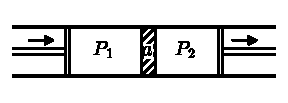
\includegraphics[width=6cm]{fig2.pdf}\\[0.3em]{\small 图 2}\end{minipage}\par\nopagebreak

上面描述的过程称为焦耳-汤姆孙过程.应当着重指出：该过程是不可逆的，这从存在具有许多小孔的壁就可以看出，它会产生很大的摩擦，把气体的速度消耗掉.

设有一定量气体在压强$P_1$下充满体积$V_1$，绝热地迁移到$V_2$中去，并且压强变为$P_2$.气体能量的变化$E_2-E_1$，等于让气体移出体积$V_1$对之所做的功$P_1V_1$，减去气体在压强$P_2$下占有体积$V_2$其所做的功$P_2V_2$.因此，有$E_2-E_1=P_1V_1-P_2V_2$，或$E_1+P_1V_1=E_2+P_2V_2$，此即
\begin{equation}
  W_1=W_2.
\end{equation}
所以，在焦耳-汤姆孙过程中，气体的焓守恒.

在压强作微小变化的情况下，焦耳-汤姆孙过程所引起的温度变化由等焓下所取的导数
$\left(\dfrac{\partial T}{\partial P}\right)_w$决定.变换这个导数，使$P$，$T$为自变量，有
\begin{equation*}
  \left(\frac{\partial T}{\partial P}\right)_w
  =\frac{\partial(T,W)}{\partial(P,W)}
  =\frac{\partial(T,W)/\partial(P,T)}
  {\partial(P,W)/\partial(P,T)}
  =-\frac{\left(\dfrac{\partial W}{\partial P}\right)_T}
  {\left(\dfrac{\partial W}{\partial T}\right)_p},
\end{equation*}
由此并借助公式(14.7)和(16.7)，得
\begin{equation}
  \left(\frac{\partial T}{\partial P}\right)_w
  =\frac{1}{C_p}\left[T\left(\frac{\partial V}{\partial T}\right)_p
  -V\right].
\end{equation}
熵的变化取决于导数
$\left(\dfrac{\partial S}{\partial P}\right)_w$.关系式
$\mathrm{d}W=T\,\mathrm{d}S+V\,\mathrm{d}P$可写成
$\mathrm{d}S=\dfrac{1}{T}\,\mathrm{d}W-\dfrac{V}{T}\,\mathrm{d}P$，由之有
\begin{equation}
  \left(\frac{\partial S}{\partial P}\right)_w=-\frac{V}{T}.
\end{equation}
这个量总是负的，这是理所当然的：因为气体经过不可逆的焦耳-汤姆孙过程而变到较低压强时伴随着熵的增加.

我们再讨论一个如下过程，最初处于两个连通容器之一的气体膨胀到第二个容器中去；这个过程当然是不稳定的，并且这两个容器中的压强都要发生变化，直到彼此相等为止.在气体膨胀到真空中时，其能量$E$守恒.如果由于膨胀的结果，总体积只有不大的变化，则温度的变化取决于导数
$\left(\dfrac{\partial T}{\partial V}\right)_E$.把这个导数变换到以$V,T$为自变量，我们得到公式
\begin{equation}
  \left(\frac{\partial T}{\partial V}\right)_E
  =\frac{1}{C_v}\left[P-T\left(\frac{\partial P}{\partial T}\right)_v\right].
\end{equation}
对于熵的变化有
\begin{equation}
  \left(\frac{\partial S}{\partial V}\right)_E=\frac{P}{T}.
\end{equation}
正如所料，气体膨胀时，熵增加.

\section{最大功}

考虑由几个彼此并不处于热平衡的物体所组成的绝热系统.在建立热平衡的过程中，系统可以（对某个外界客体）做功.然而，向平衡状态的过渡可以通过不同的方式来实现，而且系统最终的平衡状态也将是不同的；特别地，系统的能量和熵将会是不同的.

根据这一点，从不平衡的系统可能获得的总功将与建立平衡的方式有关，因而可以提出以下问题：为使系统产生尽可能大的功，向平衡状态的过渡应该如何进行.同时，我们感兴趣的正是由于系统的不平衡性所做的那部分功；这意味着必须除去由于系统一般膨胀所可能做的功——系统本身处于平衡状态也能做这样的功.根据这一点，我们将假定在过程结束时系统的总体积保持不变（虽然在过程进行之中可能有所变化）.

设系统的初始能量为$E_0$，而系统在平衡状态下的能量作为系统在该状态下熵的函数为$E(S)$.由于系统是热绝缘的，它所做的功就简单地等于其能量的变化：
\begin{equation*}
  |R|=E_0-E(S)
\end{equation*}
（我们写成$|R|$，是因为根据我们约定，如果系统本身做功，就有$R<0$）.

把$|R|$对末态的熵$S$求导数，有
\begin{equation*}
  \frac{\partial|R|}{\partial S}
  =-\left(\frac{\partial E}{\partial S}\right)_v=-T,
\end{equation*}
式中$T$是末态的温度；导数在系统末态体积（与初态值相同）恒定的条件下取.我们看到，该导数是负的，即$|R|$随着$S$的增加而减小.但是热绝缘系统的熵不可能减少.因此，只要在整个过程进行中$S$保持不变，就会达到最大可能的$|R|$.

因此，我们得出结论：当系统的熵保持不变时，即按可逆方式向平衡态过渡时，系统做的功最大.

设有两个具有不同温度$T_1$和$T_2$的物体，而且$T_2>T_1$.我们来确定当它们之间有小量的能量交换时可能产生的最大功.首先要着重指出：假如能量的转移是在两个物体相互接触时直接发生的话，那么就什么功也不会产生.这时过程将是不可逆的（两个物体的熵会增加
$\delta E\left(\dfrac{1}{T_1}-\dfrac{1}{T_2}\right)$，其中$\delta E$是转移的能量）.

因此，为了实现能量的可逆转移而相应地得到最大功，还必须把一个实现某种可逆循环过程的辅助性物体（“工作物体”）引进系统中.这个过程应该这样进行，使得彼此直接进行能量交换的物体处于相同的温度，就是说，我们在温度$T_2$下把工作物体同温度为$T_2$的物体相接触并等温地从后者获得一定的能量.随后，它被绝热地冷却到温度$T_1$，并在此温度下把能量给予温度为$T_1$的物体，最后，又绝热地返回到初态.在与这些过程相联系的膨胀过程中，工作物体对外界客体做功.以上所描述的循环过程称为卡诺循环.

在着手计算所获得的最大功时，值得指出，工作物体在这里可以不予考虑，因为过程的结果仍旧是使它返回到最初的状态.设比较热的第二个物体失去热量
$-\delta E_2=-T_2\delta S_2$，而第一个物体同时获得能量
$\delta E_1=T_1\delta S_1$.由于过程的可逆性，两个物体熵的和保持不变，即
$\delta S_1=-\delta S_2$.所做的功等于两个物体总能量的减少，即
\begin{equation*}
  |\delta R|_{\max}
  =-\delta E_1-\delta E_2
  =-T_1\delta S_1-T_2\delta S_2
  =-(T_2-T_1)\delta S_2,
\end{equation*}
或
\begin{equation}
  |\delta R|_{\max}
  =\frac{T_2-T_1}{T_2}|\delta E_2|.
\end{equation}
所做的功与所耗费的能量之比称为效率$\eta$.根据(19.1)式，当能量从较热的物体转移到较冷的物体时，最大效率等于
\begin{equation}
  \eta_{\max}=\frac{T_2-T_1}{T_2}.
\end{equation}
一个更方便的量是利用系数$n$，它定义为所做的功与在给定条件下可能获得的最大功的比.显然，
\begin{equation*}
  n=\frac{\eta}{\eta_{\max}}.
\end{equation*}

\section{处于外部介质中的物体所做的最大功}

现在我们考虑另一种情况下的最大功问题.设物体处于外部介质中，而且介质的温度$T_0$和压强$P_0$与物体的温度$T$和压强$P$并不相同.物体可以对某个客体做功，假定该客体不仅与介质，而且与该物体都是热绝缘的.介质与处于其中的物体以及物体对之做功的客体一起组成闭合系统.介质具有如此巨大的体积和能量，以致由于物体所经历的过程而引起的能量与体积的改变，不会导致介质的温度与压强有任何可觉察的变化，因而可以认为介质的温度和压强是不变的.

假如没有介质，那么在物体状态变化给定（即给定物体的初态与末态）的情况下，物体对热绝缘的客体所做的功就是一个完全确定的量，等于物体能量的变化.然而，有了介质存在而且它也参与过程，这就使得结果不再是单值的，同时产生一个问题：在物体状态变化给定的情况下，物体能够做的最大功是怎么样的.

如果物体从一个状态转变到另一个状态时，它对外部客体做功，那么物体从第二个状态逆转变到第一个状态时，某个外功源应该对物体做功.正转变伴随着物体做最大功$|R|_{\max}$，要实现与这个转变相对应的逆转变，就要求外源耗费最小功$R_{\min}$.显然，$|R|_{\max}$与$R_{\min}$这两个功彼此相同，因此有关计算它们二者问题完全等价，下面我们就讨论热绝缘的外功源对物体所做的功.

在过程进行中，物体可以同介质交换热量和功.因为我们感兴趣的只是给定的外源对物体所做的那部分功，当然就必须把介质对物体所做的功从对物体所做的总功中分出来.这样，在物体状态的某种（不一定很小的）变化下，物体能量的总的变化由三部分组成：外源对物体所做的功$R$，介质对物体所做的功以及物体从介质获得的热量.正如上面已经指出的，由于介质的尺度很大，它的温度和压强可以认为是不变的；所以它对物体所做的功是$P_0\Delta V_0$，它所放出的热量等于$-T_0\Delta S_0$（角标为0的字母属于介质，不带角标的字母属于物体）.因此，我们有：
\begin{equation*}
  \Delta E=R+P_0\Delta V_0-T_0\Delta S_0.
\end{equation*}
由于介质和物体一起的总体积保持不变，所以$\Delta V_0=-\Delta V$.其次，由于熵增长定律有$\Delta S+\Delta S_0\geqslant0$（热绝缘的外功源的熵始终不变），因此
$\Delta S_0\geqslant-\Delta S$.所以从
$R=\Delta E-P_0\Delta V_0+T_0\Delta S_0$求得
\begin{equation}
  R\geqslant\Delta E-T_0\Delta S+P_0\Delta V.
\end{equation}
在可逆过程的情况下取等号.因此，我们再次得出结论：假如转变过程是可逆的，那么实现状态的转变所耗费的功就最小（相应地，完成逆转变产生最大功）.最小功的数值取决于公式
\begin{equation}
  R_{\min}=\Delta(E-T_0S+P_0V)
\end{equation}
（$T_0$和$P_0$是常量，可以移到符号$\Delta$之外），这个功等于物理量
$E-T_0S+P_0V$的变化.显然，最大功的公式应该以相反的符号写出：
\begin{equation}
  |R|_{\max}=-\Delta(E-T_0S+P_0V),
\end{equation}
因为初态与末态交换了位置.

如果在过程进行中，物体在每一给定的时刻都处于平衡状态（当然，同介质并不处于平衡），那么对于状态的无穷小变化，可以把(20.2)式写成另外的形式：把
$\mathrm{d}E=T\,\mathrm{d}S-P\,\mathrm{d}V$代入
$\mathrm{d}R_{\min}=\mathrm{d}E-T_0\,\mathrm{d}S+P_0\,\mathrm{d}V$，求得
\begin{equation}
  \mathrm{d}R_{\min}=(T-T_0)\,\mathrm{d}S-(P-P_0)\,\mathrm{d}V.
\end{equation}
值得指出两种重要的特殊情形.如果物体的体积和温度保持不变，并且物体的温度与介质的温度相等，则从(20.2)式有$R_{\min}=\Delta(E-TS)$，或
\begin{equation}
  R_{\min}=\Delta F,
\end{equation}
即最小功等于物体自由能的变化.倘若物体的温度和压强保持不变，并且
$T=T_0$，$P=P_0$，则有
\begin{equation}
  R_{\min}=\Delta\varPhi,
\end{equation}
即外源所做的功等于物体热力学势的变化.

值得强调的是，在这两种特殊的情形下，所指的物体应该是并非处于平衡状态的物体，所以其状态并不能仅由$T$和$V$（或$P$）唯一地确定；否则这些量不变就意味着：根本没有任何过程发生.这里可以考虑在相互反应的混合物中的化学反应、溶解过程，等等.

现在假定，处于外部介质中的物体任其自然，不对它做任何功.在这个物体中将产生自发的不可逆过程，使物体趋于平衡状态.现在应该在不等式(20.1)中令$R=0$，所以有
\begin{equation}
  \Delta(E-T_0S+P_0V)\leqslant0.
\end{equation}
这意味着，物体所经历的过程，将使$E-T_0S+P_0V$这个量不断减小，直到平衡时达到最小值.

特别是，在温度$T=T_0$和压强$P=P_0$都不变的自发过程中，物体的热力学势$\varPhi$降低，而在物体的温度$T=T_0$和体积都不变的自发过程中，物体的自由能$F$将降低.这些结果曾在§15中用另一种观点得到.应该指出，这里所得出的结论实质上并非以物体的温度和体积（或压强）在整个过程中保持不变为前提；可以断言：在任何过程的开始与结束时，只要温度和压强（或体积）是相同的（而且等于介质的温度和压强），即使它们在过程的进行中是变化的，那么物体的热力学势（或自由能）将因该过程而减小.

还可以赋予最小功另外的热力学意义.设$S_t$是物体和介质的总熵；如果物体处于同介质平衡的状态，则$S_t$是它们的总能量$E_t$的函数：
\begin{equation*}
  S_t=S_t(E_t).
\end{equation*}
假设物体并不处于同介质平衡的状态，这时它们的总熵与$S_t(E_t)$的值（在它们的总能量值$E_t$相同的条件下）相差某一数量$\Delta S_t<0$.在图3中，实线表示函数$S_t(E_t)$，而竖直线段$ab$表示数量$-\Delta S_t$，水平线段$bc$表示当物体从与介质平衡的状态逆向转变到对应于点$b$的状态时总能量的变化.换而言之，该线段表示某个外源为了使物体从与介质平衡的状态进入给定状态所必须耗费的最小功.这里所说的平衡状态（图3上的$c$点），当然跟对应于给定值$E_t$的平衡状态（$a$点）并不一致.

\par\nopagebreak\noindent\begin{minipage}{\linewidth}\centering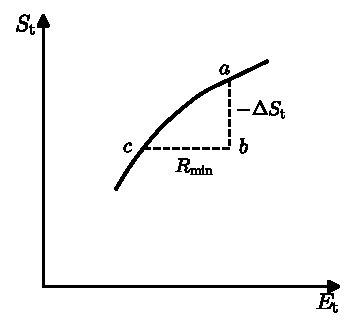
\includegraphics[width=7.5cm]{fig3.pdf}\\[0.3em]{\small 图 3}\end{minipage}\par\nopagebreak

因为物体是整个系统的一个非常小的组成部分，所以它所经历的过程只能使总能量和总熵产生相对而言极小的变化.从图3上的图形得出：
\begin{equation*}
  \Delta S_t
  =-\frac{\mathrm{d}S_t(E_t)}{\mathrm{d}E_t}R_{\min}.
\end{equation*}
但是导数$\dfrac{\mathrm{d}E_t}{\mathrm{d}S_t}$是系统的平衡温度，即介质的温度$T_0$.因此，
\begin{equation}
  \Delta S_t=-\frac{R_{\min}}{T_0}
  =-\frac{1}{T_0}(\Delta E-T_0\Delta S+P_0\Delta V).
\end{equation}
该公式确定的是：当物体并不处于同介质平衡的状态时，闭合系统（物体$+$介质）的熵与其最大可能值相差多少；这里的$\Delta E$，$\Delta S$和$\Delta V$表示物体的能量、熵和体积与它们在完全平衡状态下的值之差.

\section{热力学不等式}

从熵的极大值条件得到热平衡条件以后，直到目前，我们只考虑了熵的一阶导数.因为要求熵对能量和体积的导数为零，作为平衡条件我们得到了（§9，§12）物体所有各部分的温度和压强应该相等的条件.然而，一阶导数等于零仅仅是极值的必要条件，并不保证熵就一定取极大值.众所周知，阐明极大值的充分条件，就需要研究函数的二阶导数.

然而，不直接从闭合系统的熵为极大值的条件出发，而是从与它等效的另一个条件出发，研究这个问题更为方便\footnote{至于熵对宏观运动动量的依赖关系，则无论关于一阶导数的条件，或者关于二阶导数的条件，我们都已经研究过了（§10），其结果是求出了物体内部不存在宏观运动的要求以及温度必须大于零的要求.}.从所考虑的物体中分出某个微小的（然而是宏观的）部分.相对于这一小部分，物体的其余部分可以看成是外部的介质.这时，正如我们在上一节所见到的，能够断言，在平衡时，
\begin{equation*}
  E-T_0S+P_0V
\end{equation*}
这个量有个极小值，式中$E$，$S$，$V$是物体的该小部分的能量、熵和体积；而$T_0$，$P_0$是介质的温度和压强，即物体的其余部分的温度和压强.显然，$T_0$和$P_0$同时也是我们正研究的这一部分在平衡状态下的温度和压强.

因此，对平衡状态有任何微小的偏离时，$E-T_0S+P_0V$这个量的改变应该是正的，即
\begin{equation}
  \delta E-T_0\delta S+P_0\delta V>0.
\end{equation}
换句话说，为使物体的这一小部分从平衡状态变到任何邻近态所必须耗费的最小功应该是正的.

热力学量与其平衡值的偏差前的系数，以后都指的是平衡值，与此相应，把零角标也略去.

把$\delta E$展开为级数（把$E$看成是$S$和$V$的函数），精确到二次项，我们得到
\begin{equation*}
  \delta E=\frac{\partial E}{\partial S}\delta S
  +\frac{\partial E}{\partial V}\delta V
  +\frac{1}{2}\left(\frac{\partial^2 E}{\partial S^2}\delta S^2
  +2\frac{\partial^2 E}{\partial S\,\partial V}\delta S\,\delta V
  +\frac{\partial^2 E}{\partial V^2}\delta V^2\right).
\end{equation*}
但是$\dfrac{\partial E}{\partial S}=T$，
$\dfrac{\partial E}{\partial V}=-P$，因此这里的一次项等于
$T\delta S-P\delta V$，而且在把$\delta E$代入(21.1)式时，一次项就消去了.这样，我们得到条件
\begin{equation}
  \frac{\partial^2 E}{\partial S^2}\delta S^2
  +2\frac{\partial^2 E}{\partial S\,\partial V}\delta S\,\delta V
  +\frac{\partial^2 E}{\partial V^2}\delta V^2>0.
\end{equation}
众所周知，为使这个不等式对于任意的$\delta S$和$\delta V$都成立，必须满足下列两个条件\footnote{在(21.4)中取等号的特殊情况，将在以后的§152中考虑.}：
\begin{equation}
  \frac{\partial^2 E}{\partial S^2}>0,
\end{equation}
\begin{equation}
  \frac{\partial^2 E}{\partial S^2}
  \frac{\partial^2 E}{\partial V^2}
  -\left(\frac{\partial^2 E}{\partial S\,\partial V}\right)^2>0.
\end{equation}
因为
\begin{equation*}
  \frac{\partial^2 E}{\partial S^2}
  =\left(\frac{\partial T}{\partial S}\right)_v
  =\frac{T}{C_v},
\end{equation*}
所以条件(21.3)取$\dfrac{T}{C_v}>0$的形式，或
\begin{equation}
  C_v>0,
\end{equation}
即定容热容总是正的.

条件(21.4)可以写成雅可比行列式形式
\begin{equation*}
  \frac{\partial\left[\left(\dfrac{\partial E}{\partial S}\right)_v,
  \left(\dfrac{\partial E}{\partial V}\right)_s\right]}
  {\partial(S,V)}
  =-\frac{\partial(T,P)}{\partial(S,V)}>0.
\end{equation*}
变换到以$T$和$V$为自变量.有
\begin{equation*}
  \frac{\partial(T,P)}{\partial(S,V)}
  =\frac{\partial(T,P)/\partial(T,V)}
  {\partial(S,V)/\partial(T,V)}
  =\frac{\left(\dfrac{\partial P}{\partial V}\right)_T}
  {\left(\dfrac{\partial S}{\partial T}\right)_v}
  =\frac{T}{C_v}\left(\frac{\partial P}{\partial V}\right)_T<0.
\end{equation*}
因为$C_v>0$，上式相当于条件
\begin{equation}
  \left(\frac{\partial P}{\partial V}\right)_T<0,
\end{equation}
即在温度不变的条件下，体积的增加总是伴随着压强的减小.

条件(21.5)和(21.6)称为热力学不等式.不满足这两个条件的状态是不稳定的，因而在自然界中不可能存在.

在§16中已经指出，由于不等式(21.6)和公式(16.10)总有$C_p>C_v$，因此由(21.5)式，可得出结论，总有
\begin{equation}
  C_p>0.
\end{equation}
$C_v$和$C_p$是正的，意味着在体积不变的条件下能量是随温度单调增长的函数，而在压强不变的条件下焓也是随温度单调增长的函数.至于熵则无论在体积不变的条件下还是在压强不变的条件下，都随温度单调增长.

条件(21.5)，(21.6)是对物体中任何一个微小的部分推导出来的，因为在平衡状态下所有各部分的温度和压强彼此都相等，当然这些条件也适用于整个物体.这里我们假定物体是均匀的（至今也只考虑这样的物体）.我们着重指出，满足条件(21.5)，(21.6)正好与物体的均匀性有关.例如，可以考虑这样的物体，其粒子是靠万有引力维系在一起的；显然，这样的物体是不均匀的，它将沿着指向中心的方向逐渐变得稠密.物体的热容整体也可以小于零，即物体可以随着能量的减小而变热.值得指出，这与物体每一小部分的热容大于零的结论并不矛盾，因为在这种条件下，整个物体的能量并不等于它的各部分的能量之和——这些部分之间还存在着万有引力相互作用产生的附加能量.

我们推导出来的不等式是平衡条件.但是满足这些条件并不足以使得平衡是完全稳定的.

的确，可以存在这样的状态，当无限小地偏离该状态时，熵减小，因此物体接着就返回到初态；当产生某一有限偏离时，熵有可能比初态更大.在这种有限偏离的情况下，物体并不返回到初态，相反地，会趋向于转变到某个其它的平衡态，这个状态所对应的熵的极大值比最初状态中熵的极大值还要大.相应于这种可能性，在平衡状态中，需要区别所谓亚稳态和稳定态.如果物体处于亚稳态，则在偏离足够大时，物体可能不返回初态.虽然亚稳态在一定限度内是稳定的，但是物体迟早终究要从该状态转变到另一个稳定的状态中.后者对应于所有可能的极大熵中的最大者；离开这种状态的物体迟早会返回到这个状态.

\section{勒夏特列原理}

考虑由介质和被介质所包围的物体所组成的闭合系统.设$S$为系统的总熵，而$y$为属于物体的某一个量，并且是这样一种量：$S$相对于它具有极大值的条件$\dfrac{\partial S}{\partial y}=0$，表示物体本身处于平衡状态，而并不一定同介质处于平衡.再设$x$为属于同一物体的另一个热力学量，并且是这样一种量：如果除了$\dfrac{\partial S}{\partial y}=0$以外，还有$\dfrac{\partial S}{\partial x}=0$，则表示物体不仅处于自身的内部平衡，而且也同介质处于平衡.

引入符号
\begin{equation}
  X=-\frac{\partial S}{\partial x},\qquad
  Y=-\frac{\partial S}{\partial y}.
\end{equation}
在完全的热力学平衡状态下，熵$S$应当是极大值.因此，除条件
\begin{equation}
  X=0,\qquad Y=0,
\end{equation}
以外，还应该满足不等式
\begin{equation}
  \left(\frac{\partial X}{\partial x}\right)_y>0,\qquad
  \left(\frac{\partial Y}{\partial y}\right)_x>0,
\end{equation}
并且
\begin{equation}
  \left(\frac{\partial X}{\partial x}\right)_y
  \left(\frac{\partial Y}{\partial y}\right)_x
  -\left(\frac{\partial X}{\partial y}\right)_x^2>0.
\end{equation}
现在假定，经过某种不太大的外部作用，物体与介质的平衡被破坏，而且量$x$稍有变化，条件$X=0$也被破坏；而至于量$y$，则假定它并不受该作用的直接影响.设$\Delta x$是量$x$的变化，则在受到作用的那一时刻量$X$的变化为
\begin{equation*}
  (\Delta X)_y
  =\left(\frac{\partial X}{\partial x}\right)_y\Delta x.
\end{equation*}
在$y$不变的情况下，$x$的变化当然会破坏$Y=0$的条件，即破坏了物体内部的平衡.此后，当平衡重新恢复以后，量$X\equiv\Delta X$将取数值
\begin{equation*}
  (\Delta X)_{Y=0}
  =\left(\frac{\partial X}{\partial x}\right)_{Y=0}\Delta x,
\end{equation*}
式中导数是在等于零的恒定的$Y$值下取的.

我们比较$\Delta X$的这两个数值.利用雅可比行列式的性质，有
\begin{equation*}
  \left(\frac{\partial X}{\partial x}\right)_{Y=0}
  =\frac{\partial(X,Y)}{\partial(x,Y)}
  =\frac{\partial(X,Y)/\partial(x,y)}
  {\partial(x,Y)/\partial(x,y)}
  =\left(\frac{\partial X}{\partial x}\right)_y
  -\frac{\left(\dfrac{\partial X}{\partial y}\right)_x^2}
  {\left(\dfrac{\partial Y}{\partial y}\right)_x}.
\end{equation*}
根据条件(22.3)，在上式中第二项的分母是正的，再考虑到不等式(22.4)，求得
\begin{equation}
  \left(\frac{\partial X}{\partial x}\right)_y
  >\left(\frac{\partial X}{\partial x}\right)_{Y=0}>0,
\end{equation}
或
\begin{equation}
  |(\Delta X)_y|>|(\Delta X)_{Y=0}|.
\end{equation}
不等式(22.5)或(22.6)构成所谓勒夏特列原理的内容.

我们把量$x$的变化$\Delta x$看作为外界对物体作用的量度，而把$\Delta X$看作在这种作用的影响下物体性质变化的量度.不等式(22.6)表明，在外部作用使物体离开平衡状态以后，当物体内部的平衡又恢复时，$\Delta X$的值变小了.所以，勒夏特列原理可以表述如下：使物体离开平衡状态的外部作用，会在物体中引发一些过程，力图减弱该作用的影响.

我们举例来阐明上述内容.

首先，利用(20.8)式，把$X$和$Y$这两个量的定义稍加改变较为方便；根据(20.8)式，介质加物体所组成系统的熵的变化等于
$-\dfrac{R_{\min}}{T_0}$，式中$T_0$是介质的温度，而$R_{\min}$是把物体从与介质处于平衡的状态引到给定状态时必须做的最小功.于是可写
\begin{equation}
  X=\frac{1}{T_0}\frac{\partial R_{\min}}{\partial x},\qquad
  Y=\frac{1}{T_0}\frac{\partial R_{\min}}{\partial y}
\end{equation}
对于物体状态的无穷小变化，有（参看(20.4)）
\begin{equation*}
  \mathrm{d}R_{\min}=(T-T_0)\,\mathrm{d}S-(P-P_0)\,\mathrm{d}V;
\end{equation*}
从今以后没有下标的所有量都属于物体，而具有下标0的量都属于介质.

设$x$是物体的熵$S$，那么$X=\dfrac{T-T_0}{T_0}$.平衡条件$X=0$给出
$T=T_0$，即物体的温度与介质的温度相等.不等式(22.5)和(22.6)取形式
\begin{equation}
  \left(\frac{\partial T}{\partial S}\right)_y
  >\left(\frac{\partial T}{\partial S}\right)_{Y=0}>0,
\end{equation}
\begin{equation}
  |(\Delta T)_y|>|(\Delta T)_{Y=0}|.
\end{equation}
这些不等式的意义如下.量$x$（物体的熵）的变化表明：有一定的热量传给物体（或从物体中取出）.结果物体自身的平衡被破坏，特别是物体的温度改变了（变化了$(\Delta T)_y$）.物体内平衡的恢复导致物体温度的变化在绝对值上减小（变为$(\Delta T)_{Y=0}$），即好像使物体从平衡状态偏离作用的后果被减弱了一样.可以说，加热（冷却）物体会在物体中引发一些过程，这些过程会促使物体降低（升高）温度.

现在，设$x$是物体的体积$V$，那么
$X=-\dfrac{P-P_0}{T_0}$.平衡时$X=0$，即$P=P_0$.不等式(22.5)和(22.6)给出
\begin{equation}
  \left(\frac{\partial P}{\partial V}\right)_y
  <\left(\frac{\partial P}{\partial V}\right)_{Y=0}<0,
\end{equation}
\begin{equation}
  |(\Delta P)_y|>|(\Delta P)_{Y=0}|.
\end{equation}
如果物体（在温度不变的条件下）体积改变而偏离平衡，那么，特别是它的压强就会改变；在物体内平衡的恢复会使压强改变的绝对值减小.物体体积的减小会增加它的压强，反之亦然.注意到这一点，可以说，物体体积的减小（或增加）会在物体中引发一些过程，这些过程会促使压强减小（或增加）.

今后，我们会遇到这些结果在（溶液、化学反应等等）各方面的一系列应用.还应该指出，如果在不等式(22.8)中，取物体的体积作为量$y$，则我们有：
\begin{equation*}
  \left(\frac{\partial T}{\partial S}\right)_y
  =\left(\frac{\partial T}{\partial S}\right)_v
  =\frac{T}{C_v},\qquad
  \left(\frac{\partial T}{\partial S}\right)_{Y=0}
  =\left(\frac{\partial T}{\partial S}\right)_p
  =\frac{T}{C_p},
\end{equation*}
因为条件$Y=0$在该情况下是指$P=P_0$，即压强恒定.因此，我们再次得到熟知的不等式$C_p>C_v>0$.

类似地，如果在(22.10)中，取物体的熵作为$y$，则条件$Y=0$将表示温度是常数$T=T_0$，因而得到
\begin{equation*}
  \left(\frac{\partial P}{\partial V}\right)_s
  <\left(\frac{\partial P}{\partial V}\right)_T<0,
\end{equation*}
这也是我们已经熟知的结果.

\section{能斯特定理}

热容$C_v$大于零的这一事实表示：能量是温度的单调增长函数.反之，当温度下降时能量单调地减小，因而，在最低的可能温度即绝对零度时，物体应该处于具有最小可能能量的状态.如果假想物体划分为许多部分，把物体的能量看作这些部分的能量之和，则可以断言这些部分中的每一个也将处于能量最小的状态；显然，当总和取极小值时，它的所有各项也必然相应地取极小值.

所以，在绝对零度时，物体的任何一部分应该处于一个确定的量子态——基态.换句话说，这些部分的统计权重都等于一，因而它们的乘积，即整个物体的宏观状态的统计权重也等于一.因而，物体的熵——统计权重的对数——等于零.

因此，我们得出如下重要的结论：在绝对零度时，任何物体的熵都变为零\footnote{为避免误解，我们强调指出：凡讨论温度趋近于零都是在某些其它条件不变的情况之下——比如说在体积不变或压强不变的条件下.但是假如在使气体的温度趋近于零的同时，又无限地减小它的密度，则熵就可以不变为零.}（称为能斯特定理（W.Nernst，1906））.

值得强调的是，这个定理是量子统计学的结论，分立量子态的概念在量子统计学中起重要作用.在纯粹的经典统计学中，这个定理是不能被证明的，这时熵始终只能确定到具有一个任意附加常数的准确度（参看§7）.

能斯特定理还能够对其它某些热力学量在$T\to0$时的行为作出结论.例如，容易看出，当$T=0$时，热容——无论是$C_p$还是$C_v$——都变为零：
\begin{equation}
  \text{当~$T=0$~时，}\quad C_p-C_v=0.
\end{equation}
只要把热容的定义写成形式
\begin{equation*}
  C=T\frac{\partial S}{\partial T}
  =\frac{\partial S}{\partial\ln T},
\end{equation*}
就可以直接得出(23.1)式.当$T\to0$时，有$\ln T\to-\infty$，但因为$S$趋向于常数极限（即零），显然，上述导数趋于零.

其次，热膨胀系数变为零：
\begin{equation}
  \text{当~$T=0$~时，}\quad
  \left(\frac{\partial V}{\partial T}\right)_p=0.
\end{equation}
实际上，这个导数等于导数
$-\left(\dfrac{\partial S}{\partial P}\right)_T$（参看(16.4)），而后者在
$T=0$时变为零，因为当$T=0$时，不论压强如何，总有$S=0$.

类似地，我们可以证明：
\begin{equation}
  \text{当~$T=0$~时，}\quad
  \left(\frac{\partial P}{\partial T}\right)_v=0.
\end{equation}
通常当$T\to0$时，熵按某种幂律变为零，即$S=aT^n$，其中$a$是压强或体积的函数.显然，在这种情况下，热容和
$\left(\dfrac{\partial V}{\partial T}\right)_p$，
$\left(\dfrac{\partial P}{\partial T}\right)_v$这些量都按同样的规律（即按同样的幂次$n$）变为零.

最后，可以看出，$C_p-C_v$较之热容本身更快地变为零，即
\begin{equation}
  \text{当~$T=0$~时，}\quad
  \frac{C_p-C_v}{C_p}=0.
\end{equation}
实际上，当$T\to0$时，设熵按规律$S\propto T^n$趋近于零.从(16.9)式可以看出，这时$C_p-C_v\propto T^{2n+1}$，因此
$\dfrac{C_p-C_v}{C_p}\propto T^{n+1}$（应当注意，当$T=0$时，压缩率
$\left(\dfrac{\partial V}{\partial P}\right)_T$一般说来仍然是一个不等于零的有限值）.

如果在温度的整个变化范围内物体的热容都是已知的，则熵可以用积分的方法计算出来，而且用能斯特定理可以确定出积分常数的值.于是，在给定的压强值下，熵对温度的关系由如下公式确定
\begin{equation}
  S=\int_0^T\frac{C_p}{T}\,\mathrm{d}T,
\end{equation}
对于焓，类似的公式为
\begin{equation}
  W=W_0+\int_0^T C_p\,\mathrm{d}T,
\end{equation}
式中$W_0$是在$T=0$时焓的值.对于热力学势$\varPhi=W-TS$，相应地有
\begin{equation}
  \varPhi=W_0+\int_0^T C_p\,\mathrm{d}T
  -T\int_0^T\frac{C_p}{T}\,\mathrm{d}T.
\end{equation}

\section{热力学量对粒子数的依赖关系}

除了能量和熵以外，像$F$，$\varPhi$，$W$这些热力学量也都具有可加性（可加性可以从这些量的定义直接得出，只要考虑到压强和温度在处于平衡状态的整个物体内都是不变的）.这种可加性使我们能够对于这些量依赖于物体中粒子数的特征作出某些结论.在这里我们考虑由相同粒子（分子）构成的物体；所有的结果都能直接推广到由不同粒子所构成的物体——混合物上去（参看§83）.

物理量的可加性意味着：物质的数量（与其相关的就是粒子数$N$）变化了多少倍，则该物理量也变化多少倍.换句话说，可加性的热力学量应该是可加性变量的一次齐次函数.

我们把物体的能量表示为熵和体积以及粒子数的函数.因为$S$和$V$本身也是可加性的，这个函数应该取如下形式：
\begin{equation}
  E=Nf\left(\frac{S}{N},\frac{V}{N}\right),
\end{equation}
这是$N$，$S$和$V$的一次齐次函数的最普遍的形式.自由能$F$是$N$，$T$和$V$的函数.因为温度在整个物体内部都是不变的，而体积是可加性的，所以出于同样的考虑，可以写出
\begin{equation}
  F=Nf\left(\frac{V}{N},T\right).
\end{equation}
完全类似地，把焓$W$表示为$N$，$S$和压强$P$的函数形式，我们得到
\begin{equation}
  W=Nf\left(\frac{S}{N},P\right).
\end{equation}
最后，对于作为$N$，$P$，$T$的函数的热力学势，有
\begin{equation}
  \varPhi=Nf(P,T)
\end{equation}
在以上的叙述中，实质上我们是把粒子数看作是一个参量，对于每一个物体它具有给定的常数值.现在，我们在形式上把$N$也看成是一个自变量.那么在热力学势的微分表达式中，应该附加一个正比于$\mathrm{d}N$的项.例如，我们把能量的全微分写成
\begin{equation}
  \mathrm{d}E=T\,\mathrm{d}S-P\,\mathrm{d}V+\mu\,\mathrm{d}N,
\end{equation}
式中我们用字母$\mu$表示偏导数
\begin{equation}
  \mu=\left(\frac{\partial E}{\partial N}\right)_{s,v},
\end{equation}
$\mu$这个量称为物体的化学势.类似地，用同样的$\mu$，现在有
\begin{equation}
  \mathrm{d}W=T\,\mathrm{d}S+V\,\mathrm{d}P+\mu\,\mathrm{d}N,
\end{equation}
\begin{equation}
  \mathrm{d}F=-S\,\mathrm{d}T-P\,\mathrm{d}V+\mu\,\mathrm{d}N,
\end{equation}
\begin{equation}
  \mathrm{d}\varPhi=-S\,\mathrm{d}T+V\,\mathrm{d}P+\mu\,\mathrm{d}N.
\end{equation}
从这些公式中得出
\begin{equation}
  \mu=\left(\frac{\partial W}{\partial N}\right)_{s,p}
  =\left(\frac{\partial F}{\partial N}\right)_{T,v}
  =\left(\frac{\partial\varPhi}{\partial N}\right)_{p,T},
\end{equation}
也就是说，把$E$，$W$，$F$，$\varPhi$这些量中的任何一个对粒子数求导数，就可以得到化学势，但是在每一种情形下化学势是用不同的变量来表示的.

把写成(24.4)形式的$\varPhi$进行微分，我们求出
$\mu=\dfrac{\partial\varPhi}{\partial N}=f(P,T)$，即
\begin{equation}
  \varPhi=N\mu.
\end{equation}
由此可见，（由相同粒子所构成的）物体的化学势不是别的，而是属于一个分子的热力学势.化学势可以表示为$P$和$T$的函数，而与$N$无关.因此，对化学势的微分而言，可以立即写出如下表达式
\begin{equation}
  \mathrm{d}\mu=-s\,\mathrm{d}T+v\,\mathrm{d}P,
\end{equation}
式中$s$和$v$是属于一个分子的熵和体积.

如果考虑一定量的物质（直到目前为止，我们通常都是这么做的），则其中的粒子数是给定的常量，而它的体积是变量.现在我们在物体内划分出某个一定的体积，并考虑这个体积中所包含的物质；在这种情况下，粒子数$N$将是变量，而体积$V$将是常量.这时，例如等式(24.8)就化为
\begin{equation*}
  \mathrm{d}F=-S\,\mathrm{d}T+\mu\,\mathrm{d}N.
\end{equation*}
在这里自变量是$T$和$N$；我们引入这样一种热力学势：它的第二个自变量不是$N$，而是$\mu$.为此把
$\mu\,\mathrm{d}N=\mathrm{d}(\mu N)-N\,\mathrm{d}\mu$代入，就得到
\begin{equation*}
  \mathrm{d}(F-\mu N)=-S\,\mathrm{d}T-N\,\mathrm{d}\mu.
\end{equation*}
但是，$\mu N=\varPhi$，而$F-\varPhi=-PV$.所以，一种新的热力学势（我们用字母$\Omega$来表示它）就等于
\begin{equation}
  \Omega=-PV
\end{equation}
而且
\begin{equation}
  \mathrm{d}\Omega=-S\,\mathrm{d}T-N\,\mathrm{d}\mu
\end{equation}
在温度和体积都不变的条件下，把$\Omega$对化学势求导数，就得到粒子数.
\begin{equation}
  N=-\left(\frac{\partial\Omega}{\partial\mu}\right)_{T,v}
  =V\left(\frac{\partial P}{\partial\mu}\right)_{T,v}
\end{equation}
就像证明$E$，$W$，$F$和$\varPhi$（各自在相应的一对变量恒定时）的小增量彼此相等一样，容易证明在$T$，$\mu$，$V$不变的条件下，变化
$(\delta\Omega)_{T,\mu,v}$也具有相同的性质.换句话说，
\begin{equation}
  (\delta E)_{s,v,N}=(\delta F)_{T,v,N}
  =(\delta\varPhi)_{T,p,N}=(\delta W)_{s,p,N}
  =(\delta\Omega)_{T,v,\mu}.
\end{equation}
这些等式改进并推广了小增量定理.

最后，类似于在§15和§20中对自由能和热力学势所进行的推导，可以证明，在$T$，$V$和$\mu$不变的条件下所进行的一个可逆过程中所做的功，就等于热力学势$\Omega$的变化.相对于状态在$T,V,\mu$不变的条件下的一切变化，在热平衡状态下的势$\Omega$有极小值.

\begin{xiti}

试求在变量取$T$，$\mu$，$V$时热容$C_v$的表达式.

解：把导数
$C_v=T\left(\dfrac{\partial S}{\partial T}\right)_{v,N}$变换到以$T,V$和$\mu$作为自变量，为此，我们写出（考虑$V$始终不变）：
\begin{equation*}
  \left(\frac{\partial S}{\partial T}\right)_N
  =\frac{\partial(S,N)}{\partial(T,N)}
  =\frac{\partial(S,N)/\partial(T,\mu)}
  {\partial(T,N)/\partial(T,\mu)}
  =\left(\frac{\partial S}{\partial T}\right)_\mu
  -\frac{\left(\dfrac{\partial S}{\partial\mu}\right)_T
  \left(\dfrac{\partial N}{\partial T}\right)_\mu}
  {\left(\dfrac{\partial N}{\partial\mu}\right)_T}.
\end{equation*}
但是
$\left(\dfrac{\partial S}{\partial\mu}\right)_T
=-\dfrac{\partial^2\Omega}{\partial T\,\partial\mu}
=\left(\dfrac{\partial N}{\partial T}\right)_\mu$；所以
\begin{equation*}
  C_v=T\left[\left(\frac{\partial S}{\partial T}\right)_\mu
  -\frac{\left(\dfrac{\partial N}{\partial T}\right)_\mu^2}
  {\left(\dfrac{\partial N}{\partial\mu}\right)_T}\right].
\end{equation*}

\end{xiti}

\section{在外场中物体的平衡}

考虑处于（时间上）恒定的外场中的物体.这时，物体的各个部分处于不同的条件下，因此物体是不均匀的.这样的物体的平衡条件之一仍旧是在整个物体中温度为常量；但是在物体中的不同地点压强是不同的.

为了推导第二个平衡条件，我们从物体中划分出两个确定的相互接触的体积，并且要求在物体的其余部分的状态不变的条件下它们的熵$S=S_1+S_2$极大.熵为极大值的必要条件之一是导数
$\dfrac{\partial S}{\partial N_1}$等于零.因为在给定的物体这两部分中的粒子总数$N_1+N_2$可看作常数，我们有
\begin{equation*}
  \frac{\partial S}{\partial N_1}
  =\frac{\partial S_1}{\partial N_1}
  +\frac{\partial S_2}{\partial N_2}
  \frac{\partial N_2}{\partial N_1}
  =\frac{\partial S_1}{\partial N_1}
  -\frac{\partial S_2}{\partial N_2}=0.
\end{equation*}
但是只要把恒等式$\mathrm{d}E=T\,\mathrm{d}S+\mu\,\mathrm{d}N$改写成为如下形式
\begin{equation*}
  \mathrm{d}S=\frac{\mathrm{d}E}{T}
  -\frac{\mu}{T}\,\mathrm{d}N,
\end{equation*}
我们就可以看出，（在$E$和$V$恒定的条件下）导数$\dfrac{\partial S}{\partial N}$等于$-\dfrac{\mu}{T}$.因此，有
$\dfrac{\mu_1}{T_1}=\dfrac{\mu_2}{T_2}$.但是在平衡时$T_1=T_2$，因此
$\mu_1=\mu_2$.于是，我们得出以下结论：物体在外场中平衡时，除了温度为常数外，还应该遵守条件
\begin{equation}
  \mu=\text{常数，}
\end{equation}
即物体所有各部分的化学势应该彼此相等.这时，每一部分的化学势是它的温度和压强的函数，也是确定外场的诸参量的函数.如果没有外场，则由$\mu$和$T$为常数的条件，自动地得出压强也为常数.

在引力场中，分子的势能$u$只是其重心坐标$x$，$y$，$z$的函数（而与分子内原子的位置无关）.在这种情况下，物体的热力学量的变化归结为在其能量上再附加上分子在引力场中的势能.例如，化学势（属于一个分子的热力学势）取$\mu=\mu_0+u(x,y,z)$的形式，式中$\mu_0(P,T)$是没有外场时的化学势.因此，引力场中的平衡条件可以写成
\begin{equation}
  \mu_0(P,T)+u(x,y,z)=\text{常数.}
\end{equation}
特别是，在均匀的重力场中，$u=mgz$（$m$为分子的质量，$g$为重力加速度，$z$为铅直坐标）.把等式(25.2)在不变的温度条件下对坐标$z$进行微分，得到
\begin{equation*}
  v\,\mathrm{d}P=-mg\,\mathrm{d}z.
\end{equation*}
式中$v=\left(\dfrac{\partial\mu_0}{\partial P}\right)_T$是比体积.在压强变化不大的条件下，$v$可以认为是不变的.引入密度$\rho=\dfrac{m}{v}$，并进行积分，得到
\begin{equation*}
  P=\text{常数}-\rho gz,
\end{equation*}
这就是在不可压缩的液体中通常的流体静压强的公式.

\section{转动的物体}

正如我们在§10中已经看到的，在热平衡状态，只有物体整体的匀速平动和匀速转动才有可能.对于匀速平动无需作任何特殊的讨论，因为根据伽利略相对性原理，它无论如何也不会影响物体的力学性质，所以也不会影响物体的热力学性质，而且，说物体的热力学量有变化，也只是在物体的能量上附加了物体的动能.

现在考虑以角速度$\boldsymbol{\Omega}$围绕一根固定轴作匀速转动的物体.设$E(\boldsymbol{p},\boldsymbol{q})$是物体在静止坐标系中的能量，而
$E'(\boldsymbol{p},\boldsymbol{q})$是在随物体一起转动的坐标系中的能量.从力学中已经知道，这两个能量通过如下关系彼此相联系：
\begin{equation}
  E'(\boldsymbol{p},\boldsymbol{q})
  =E(\boldsymbol{p},\boldsymbol{q})
  -\boldsymbol{\Omega}\cdot\boldsymbol{M}(\boldsymbol{p},\boldsymbol{q}),
\end{equation}
式中$\boldsymbol{M}(\boldsymbol{p},\boldsymbol{q})$是物体的角动量\footnote{参看第一卷§39.虽然在那里导出的公式(39.13)是以经典力学为基础的，但是在量子理论中，对于相应各量的算符，完全同样的关系式也成立.因此，下面所导出的全部热力学关系式与用哪一种力学来描述物体粒子的运动无关.}.

因此，能量$E'(\boldsymbol{p},\boldsymbol{q})$以角速度$\boldsymbol{\Omega}$作为参量而与其有关，并且
\begin{equation*}
  \frac{\partial E'(\boldsymbol{p},\boldsymbol{q})}
  {\partial\boldsymbol{\Omega}}
  =-\boldsymbol{M}(\boldsymbol{p},\boldsymbol{q}).
\end{equation*}
将上式按统计分布求平均，并利用公式(11.3)，得到
\begin{equation}
  \left(\frac{\partial E'}{\partial\boldsymbol{\Omega}}\right)_s
  =-\boldsymbol{M},
\end{equation}
式中$E'=\overline{E'(\boldsymbol{p},\boldsymbol{q})}$，
$\boldsymbol{M}=\overline{\boldsymbol{M}(\boldsymbol{p},\boldsymbol{q})}$
是物体的平均（热力学）能量和平均角动量.

根据这个关系式，我们可以把给定体积下转动物体能量的微分写成
\begin{equation}
  \mathrm{d}E'=T\,\mathrm{d}S-\boldsymbol{M}\cdot\mathrm{d}\boldsymbol{\Omega}.
\end{equation}
对于（在转动坐标系中的）自由能$F'=E'-TS$，相应地有
\begin{equation}
  \mathrm{d}F'=-S\,\mathrm{d}T-\boldsymbol{M}\cdot\mathrm{d}\boldsymbol{\Omega}.
\end{equation}
将等式(26.1)求平均，得到
\begin{equation}
  E'=E-\boldsymbol{M}\cdot\boldsymbol{\Omega},
\end{equation}
把该等式微分，并将(26.3)式代入，就得到在静止坐标系中能量的微分
\begin{equation}
  \mathrm{d}E=T\,\mathrm{d}S+\boldsymbol{\Omega}\cdot\mathrm{d}\boldsymbol{M}.
\end{equation}
对于自由能$F=E-TS$，相应地有
\begin{equation}
  \mathrm{d}F=-S\,\mathrm{d}T+\boldsymbol{\Omega}\cdot\mathrm{d}\boldsymbol{M}.
\end{equation}
由此可见，在这些关系式中，自变量并非角速度，而是角动量，而且
\begin{equation}
  \boldsymbol{\Omega}
  =\left(\frac{\partial E}{\partial\boldsymbol{M}}\right)_s
  =\left(\frac{\partial F}{\partial\boldsymbol{M}}\right)_T
\end{equation}
从力学中大家知道，匀速转动在一定意义下等效于呈现两个力场：离心力场和科里奥利力场.离心力与物体的大小（其中包含到转动轴的距离）成正比；而科里奥利力与物体的大小完全无关.由于这种情况，后者对宏观转动物体的热力学性质的影响与前者相较十分微小，通常可以把它们完全忽略不计\footnote{可以证明：在经典统计学中，科里奥利力完全不影响物体的统计性质——参看§34.}.因此，只要把粒子的离心能量作为$u(x,y,z)$代入(25.2)式，就得到转动物体的热平衡条件：
\begin{equation}
  \mu_0(P,T)-\frac{m\Omega^2r^2}{2}=\text{常数，}
\end{equation}
式中$\mu_0$是静止物体的化学势，$m$为分子的质量，$r$为到转动轴的距离.根据同样的理由，可以把转动物体的总能量$E$写成它的内能（在这里我们用$E_{\mathrm{in}}$来代表它）与转动动能之和：
\begin{equation}
  E=E_{\mathrm{in}}+\frac{M^2}{2I},
\end{equation}
式中$I$是物体相对于转动轴的转动惯量.必须注意，一般说来，转动会改变物体中的质量分布，所以物体的转动惯量和内能一般来讲，也与$\Omega$（或与$M$）有关.只有在转动足够缓慢的情况下，这两个量才可以认为是与$\boldsymbol{\Omega}$无关的常数.

考虑孤立的匀速转动的固体，固体内部具有给定的质量分布.因为物体的熵是它的内能的函数，所以在这种情况下有
\begin{equation*}
  S=S\left(E-\frac{M^2}{2I}\right).
\end{equation*}
由于物体的闭合性，它的总能量和角动量守恒，而熵应该在给定的$M$和$E$下取极大的可能值.所以我们得出结论：物体的转动惯量相对哪一根轴具有最大的可能值，它的平衡转动就绕哪一根轴进行.这就自动地意味着：在任何情况下，转动轴总是物体的惯量主轴.其实上述情况，早就很显然，如果物体并非绕惯量主轴转动，则从力学可知，转动轴本身将在空间发生移动（进动），即转动是非均匀的，因而也是非平衡的.

\section{相对论范围内的热力学关系式}

相对论力学使通常的热力学关系式产生一系列的变化.在这里，我们只考虑那些最感兴趣的变化.

如果构成物体的粒子的微观运动变为相对论性运动，那么热力学的普遍关系式并不改变，但是能得出物体的压强与能量之间的一个重要的不等式
\begin{equation}
  P<\frac{E}{3V},
\end{equation}
式中$E$是物体的能量，其中包括构成物体的粒子的静止能量\footnote{参看第二卷§35.但是值得注意，关于该不等式适用于在自然界中所有存在的粒子间相互作用类型（不仅仅限于电磁的相互作用），目前还没有普遍证明.}.

考虑到物体自身所产生的引力场，广义相对论可引起热平衡条件中的某些变化，这些变化就是我们主要兴趣所在.考虑一个静止的宏观物体，当然，它的引力场是不变的.在恒定的引力场中，必须把物体任何一小部分的守恒能量$E_0$与位于给定位置的观察者所测量到的能量$E$区别开来.这两个量由关系式
\begin{equation*}
  E_0=E\sqrt{g_{00}}
\end{equation*}
彼此相联系，式中$g_{00}$是度规张量的时间分量（参看第二卷§88的公式(88.9)，式中$v=0$，$mc^2=E$）.但是，在§9中证明了处于平衡状态的整个物体内温度是恒定的，但是按照这个证明本来的含义，很显然，熵对守恒能量$E_0$求微商而得到的量应该是不变的.而由位于空间给定的一点的观察者测量到的温度$T$，是熵对能量$E$求微商得到的，因而在物体的不同点是各不相同的.

为导出定量的关系式，应当注意：按照熵的定义的实质，熵只与物体的内部状态有关，所以不会在出现引力场的情况下发生变化（只要在这个场不影响物体的内部性质，这一条件事实上总能满足）.因此守恒能量$E_0$对熵的导数等于$T\sqrt{g_{00}}$，由此可见，热平衡条件之一是要求该量在整个物体内为常数\footnote{方程(27.2)在$g_{00}$变为零的那些点失去意义.这种情形发生在所谓黑洞的附近.（参见第二卷§102）.这类客体热力学性质的讨论可参阅论文集：黑洞.M.；Мир，1978.}
\begin{equation}
  T\sqrt{g_{00}}=\text{常数.}
\end{equation}
第二个平衡条件——化学势恒定——也以类似的方式发生变化.化学势被定义为能量对粒子数的导数.由于粒子数当然不会因为有引力场而发生变化，所以对于在每一给定点测量到的化学势，我们得到与温度的关系式完全相似的关系式：
\begin{equation}
  \mu\sqrt{g_{00}}=\text{常数.}
\end{equation}
我们注意到，关系式(27.2)，(27.3)可以写成
\begin{equation}
  T=\text{常数}\cdot\frac{\mathrm{d}x^0}{\mathrm{d}s}\text{，}\qquad
  \mu=\text{常数}\cdot\frac{\mathrm{d}x^0}{\mathrm{d}s}\text{，}
\end{equation}
这两个式子不仅能考虑物体在参照系中静止的情况，而且也能考虑物体在参照系中运动（整体转动）的情形.这时，导数
$\dfrac{\mathrm{d}x^0}{\mathrm{d}s}$应该是沿着物体中给定点所描出的世界线来求取.

在微弱的（牛顿的）引力场中，$g_{00}=1+\dfrac{2\varphi}{c^2}$，其中$\varphi$是引力势（参看第二卷§87）.把这个式子代入(27.2)中并求出平方根，我们就在同样的近似程度下求出
\begin{equation}
  T=\text{常数}\cdot\left(1-\frac{\varphi}{c^2}\right).
\end{equation}
注意到$\varphi<0$，我们得出：当平衡时，在物体中$|\varphi|$越大的地方，即在物体中越深的地方，温度就越高.当过渡到非相对论力学的极限情形时（$c\to\infty$），(27.5)变为$T=$常数，这正是所预期的.

条件(27.3)也可以用类似的方式来变换，但是必须注意，在过渡到经典力学的极限情形时，相对论性的化学势并不直接变换到通常没有引力场时的（非相对论性的）化学势表示式，我们用字母$\mu_0$来标记，而是变为$\mu_0+mc^2$，其中$mc^2$是物体单个粒子的静止能量.因此我们有
\begin{equation*}
  \mu\sqrt{g_{00}}
  \approx(\mu_0+mc^2)\left(1+\frac{\varphi}{c^2}\right)
  \approx\mu_0+mc^2+m\varphi,
\end{equation*}
所以条件(27.3)变为
\begin{equation*}
  \mu_0+m\varphi=\text{常数，}
\end{equation*}
它与(25.2)一致，这正是所预期的.

最后，我们指出一个有用的关系式，它是条件(27.2)和(27.3)的直接推论.

把这两个表达式相除，求出$\dfrac{\mu}{T}=$常数，由此得出
$\dfrac{\mathrm{d}\mu}{\mu}=\dfrac{\mathrm{d}T}{T}$.另一方面，根据(24.12)式，在恒定的体积（等于单位体积）下，有
\begin{equation*}
  \mathrm{d}P=S\,\mathrm{d}T+N\,\mathrm{d}\mu,
\end{equation*}
式中$S$，$N$是单位体积内物体的熵和粒子数.把
$\mathrm{d}T=\dfrac{T}{\mu}\,\mathrm{d}\mu$代入上式，并注意到
$\mu N+ST=\varPhi+ST=\varepsilon+P$（$\varepsilon$是单位体积物体的能量），我们得到所求的关系式\footnote{在非相对论的情形下，令$\mu\approx mc^2$，$\varepsilon\approx\rho c^2\gg P$（$\rho$为密度），我们得到$\mathrm{d}\mu=v\,\mathrm{d}P$（$v=\dfrac{m}{\rho}$表示一个粒子所占的体积），这正如在$T=$常数时所预期的.}
\begin{equation}
  \frac{\mathrm{d}\mu}{\mu}
  =\frac{\mathrm{d}P}{\varepsilon+P}.
\end{equation}
